\documentclass{unina_delivery_class}

\begin{document}


\color{TERTIARY}

% Title page

\pagecolor{TERTIARY}\afterpage{\nopagecolor}
\begin{titlepage}
  \begin{center}
    \vspace*{0.8cm}
    \Huge
    \textbf{\maintitle{}}

    \vspace*{0.5cm}

    \color{SECONDARY}
    \large
    \textbf{\authors{}}
    
    \vfill

    
\includegraphics[width=0.8\textwidth]{UninaDelivery_logo.png}
    
    \vfill

    \vspace*{0.5cm}
    
\includegraphics[width=0.7\textwidth]{DIETI_logo.pdf}
    \vspace*{-0.5cm}
  \end{center}
\end{titlepage}

% Table of contents
\tableofcontents{}
\lstlistoflistings{}

  % Chapter 1 - "Considerazioni sul Dominio"
  \chapter{Considerazioni sul Dominio}

\section{Analisi del Problema}

Si vuole progettare e sviluppare un database per la gestione della logistica delle spedizioni di merci.

Questo sistema deve essere in grado di gestire le informazioni relative ai clienti, ai mezzi di trasporto, ai corrieri, ai magazzini e ai prodotti, per poter essere a disposizione di un operatore incaricato alla pianificazione di spedizioni.

\section{Assunzioni sul Dominio} 

Per modellare il mini-mondo relativo al problema, si sono fatte le seguenti assunzioni:

\begin{itemize}
  \item \textbf{Il sistema gestisce spedizioni di merci presenti nei propri magazzini, verso clienti che hanno effettuato un ordine}.
  
  Si è assunto che la ditta a cui è rivolto il sistema non si occupi di spedizioni postali tra clienti, ma solo di spedizioni di merci presenti nei propri magazzini, che siano della ditta stessa o lasciate in gestione alla ditta da aziende terze.

  Quest'assunzione è stata fatta per avere una linea di continuità col requisito di controllo della disponibilità della merce, cosa di cui non si occupa un servizio postale.

  \item  \textbf{Il sistema si occupa della gestione delle spedizioni verso magazzini, oltre che verso clienti}.
  
  Si è assunto che la ditta a cui è rivolto il sistema possa avere la merce richiesta da un cliente distribuita in più magazzini, e che sia sconvenevole far partire spedizioni dirette verso il cliente da ogni magazzino che ha la merce richiesta.

  Si è quindi piuttosto presupposto un sistema di spedizioni intermedie per merci che non sono presenti nel magazzino più vicino al cliente, ma che sono presenti in altri magazzini della ditta.

  \item \textbf{Il sistema non si occupa di selezionare il percorso della merce dal magazzino originario al cliente}.
  
  Si è assunto che sia compito di un operatore  selezionare il percorso della merce dal magazzino originario al cliente, e che il sistema si occupi solo di gestire le informazioni relative alla spedizione.

  Si è quindi presupposto che una merce possa andare da un magazzino a potenzialmente qualsiasi altro, e che sarà premura di un operatore scegliere percorsi ragionevoli.

  Quest'assunzione è stata fatta in funzione del requisito della traccia che richiede di far gestire all'operatore la pianificazione delle spedizioni, che chiaramente comprende anche il percorso.

  \newpage
  \item \textbf{Struttura gerarchica dei magazzini}.
  
  Si è assunto, oltre alla presenza di molteplici magazzini di proprietà della ditta, che questi magazzini siano organizzati in una struttura gerarchica territoriale come segue:
  \begin{itemize}
    \item Ogni magazzino è \textbf{cittadino}, e può spedire direttamente ai clienti della sua città.
    \item Alcuni magazzini \textbf{cittadini} sono \textbf{regionali}, che smistano le merci in una regione.
    \item Alcuni magazzini \textbf{regionali} sono \textbf{nazionali}, che smistano le merci in una nazione.
    \item Alcuni magazzini \textbf{nazionali} sono \textbf{centrali}, che smistano le merci in un continente.
    \end{itemize}

  \item \textbf{Distribuzione mezzi di trasporto}.
  
  Si è assunto che la ditta abbia a disposizione diversi tipi e livelli di mezzi per il trasporto merci, e che questi mezzi siano distribuiti in maniera diversa fra i magazzini, in base alla loro dimensione e al loro ruolo nella struttura gerarchica.

  In particolare, si è deciso di dividere i mezzi di trasporto in:
  
  \begin{itemize}
    \item \textbf{Su strada}, come camion e furgoni, divisi a loro volta in:
      \begin{itemize}
        \item \textbf{Piccoli}, ovvero furgoncini, camion di piccole dimensioni e motocicli che possono essere guidati con una patente A o B, presenti in tutti i magazzini. Ogni mezzo \textbf{su strada piccolo} può coprire una zona comprendente diversi CAP, ed è impiegato in viaggi \textbf{cittadini e intraregionali} per raggiungere il cliente finale.
        \item \textbf{Grandi}, ovvero TIR e camion di grandi dimensioni, che possono essere guidati con una patente C, presenti in magazzini regionali o superiori, per il trasporto fra magazzini, in viaggi \textbf{interregionali e intranazionali}.
      \end{itemize}
    
    \item \textbf{Su ferro}, come treni e tram, presenti in magazzini nazionali o superiori, per il trasporto fra magazzini, in viaggi \textbf{internazionali e intracontinentali}.
    
    \item \textbf{Via acqua}, come navi, presenti solo nei magazzini centrali, per il trasporto fra magazzini, in viaggi \textbf{intercontinentali}.
    
    \item \textbf{Via aria}, come aerei, presenti solo nei magazzini centrali, per il trasporto fra magazzini, in viaggi \textbf{intercontinentali}.
  
  \end{itemize}

  \item \textbf{Gestione dei trasportatori}.
  
  Si è assunto che la ditta abbia diretta responsabilità solo sui mezzi su strada, e che i mezzi su ferro, via acqua e via aria siano di enti di spedizione terzi, con cui la ditta ha un contratto di collaborazione e per questo ne conserva solo l'eventuale disponibilità e i dati a essa relativi.

  Si è dunque presupposto che gli unici trasportatori dipendenti dalla ditta siano i conducenti dei mezzi su strada, dei quali il sistema terrà traccia, tra le altre cose, della tipologia di patente, per associarli ai mezzi che possono guidare.

  \item \textbf{Gestione di ordini e spedizioni}.
  
  Si è assunto che il cliente della ditta possa effettuare un ordine contenenti più prodotti, e che la ditta possa spedire i prodotti di un ordine in più spedizioni, in base alla disponibilità dei prodotti nei magazzini.

  Si è presupposto dunque che il sistema non si occupi di gestire le spedizione in modo da evitare ritardi sulle date di consegna, ma esclusivamente di presentare in ordine le spedizioni per permettere all'operatore che pianifica le spedizioni di scegliere percorsi che evitino ritardi.

\end{itemize}

% TODO: @zGenny UML and ER diagrams needs to be updated according to the new domain assumptions


  % Chapter 2 - "Progettazione Concettuale"
  \chapter{Progettazione Concettuale}

\section{Premesse alla lettura dei diagrammi}

\subsection{Modelli Utilizzati}

Procediamo alla modellizzazione del mini-mondo, partendo dalla progettazione concettuale.

Questa fase di progettazione è stata svolta utilizzando, oltre che il modello \textbf{UML} nella forma di un \textbf{Class Diagram}, anche il modello \textbf{EER}, ovvero \textbf{Enhanced Entity Relationship}, per cogliere meglio aspetti del dominio che un modello \textbf{ER} classico non avrebbe potuto cogliere, come ad esempio \textbf{generalizzazioni e specializzazioni}.

\subsection{Precisazioni sui Diagrammi}

\subsubsection{EER Diagram}

Vista la densità del diagramma \textbf{EER}, si è deciso d'introdurre un \textbf{color coding} per facilitarne la lettura:

\begin{itemize}
  \item \textcolor{PRIMARY}{Entità}, e dunque Specializzazioni in \textcolor{PRIMARY}{arancione};
  \item \textcolor{CONTRAST}{Relazioni} in \textcolor{CONTRAST}{celeste};
  \item \textcolor{NEWGREEN}{Attributi} in \textcolor{NEWGREEN}{verde};
\end{itemize}

Inoltre, in caso di accavallamento di linee, si è deciso d'interrompere la linea in secondo piano in corrispondenza di un intersezione, così da evidenziare i diversi collegamenti.

\subsubsection{UML Class Diagram}

Per migliorare la leggibilità dei diagrammi, si è deciso di specificare le \textbf{molteplicità} degli attributi esclusivamente per sottolineare la possibilità di essere valorizzato a \textbf{NULL}. 

In tali casi si è utilizzata la molteplicità \textbf{[\(0..1\)]} esclusivamente per gli attributi di tipo \textbf{Bool}, mentre \textbf{[\(0..*\)]} per gli altri.

\bigskip

\begin{note}[Leggibilità dei Diagrammi]
  In caso di problemi di leggibilità dei diagrammi, sono disponibili le versioni originali nella pagina GitHub del progetto:
  \exlink{https://github.com/RiccardoElena/UninaDelivery/blob/develop/db/docs/sources/ER_Diagram.pdf}{ER Diagram} e \exlink{https://github.com/RiccardoElena/UninaDelivery/blob/develop/db/docs/sources/UML_Class_Diagram.pdf}{UML Class Diagram}.
\end{note}

\newpage
% TODO @zGenny export the ER diagram with the new changes and uncommend this part

\section{Enhanced Entity Relationship Diagram}
\begin{center}
  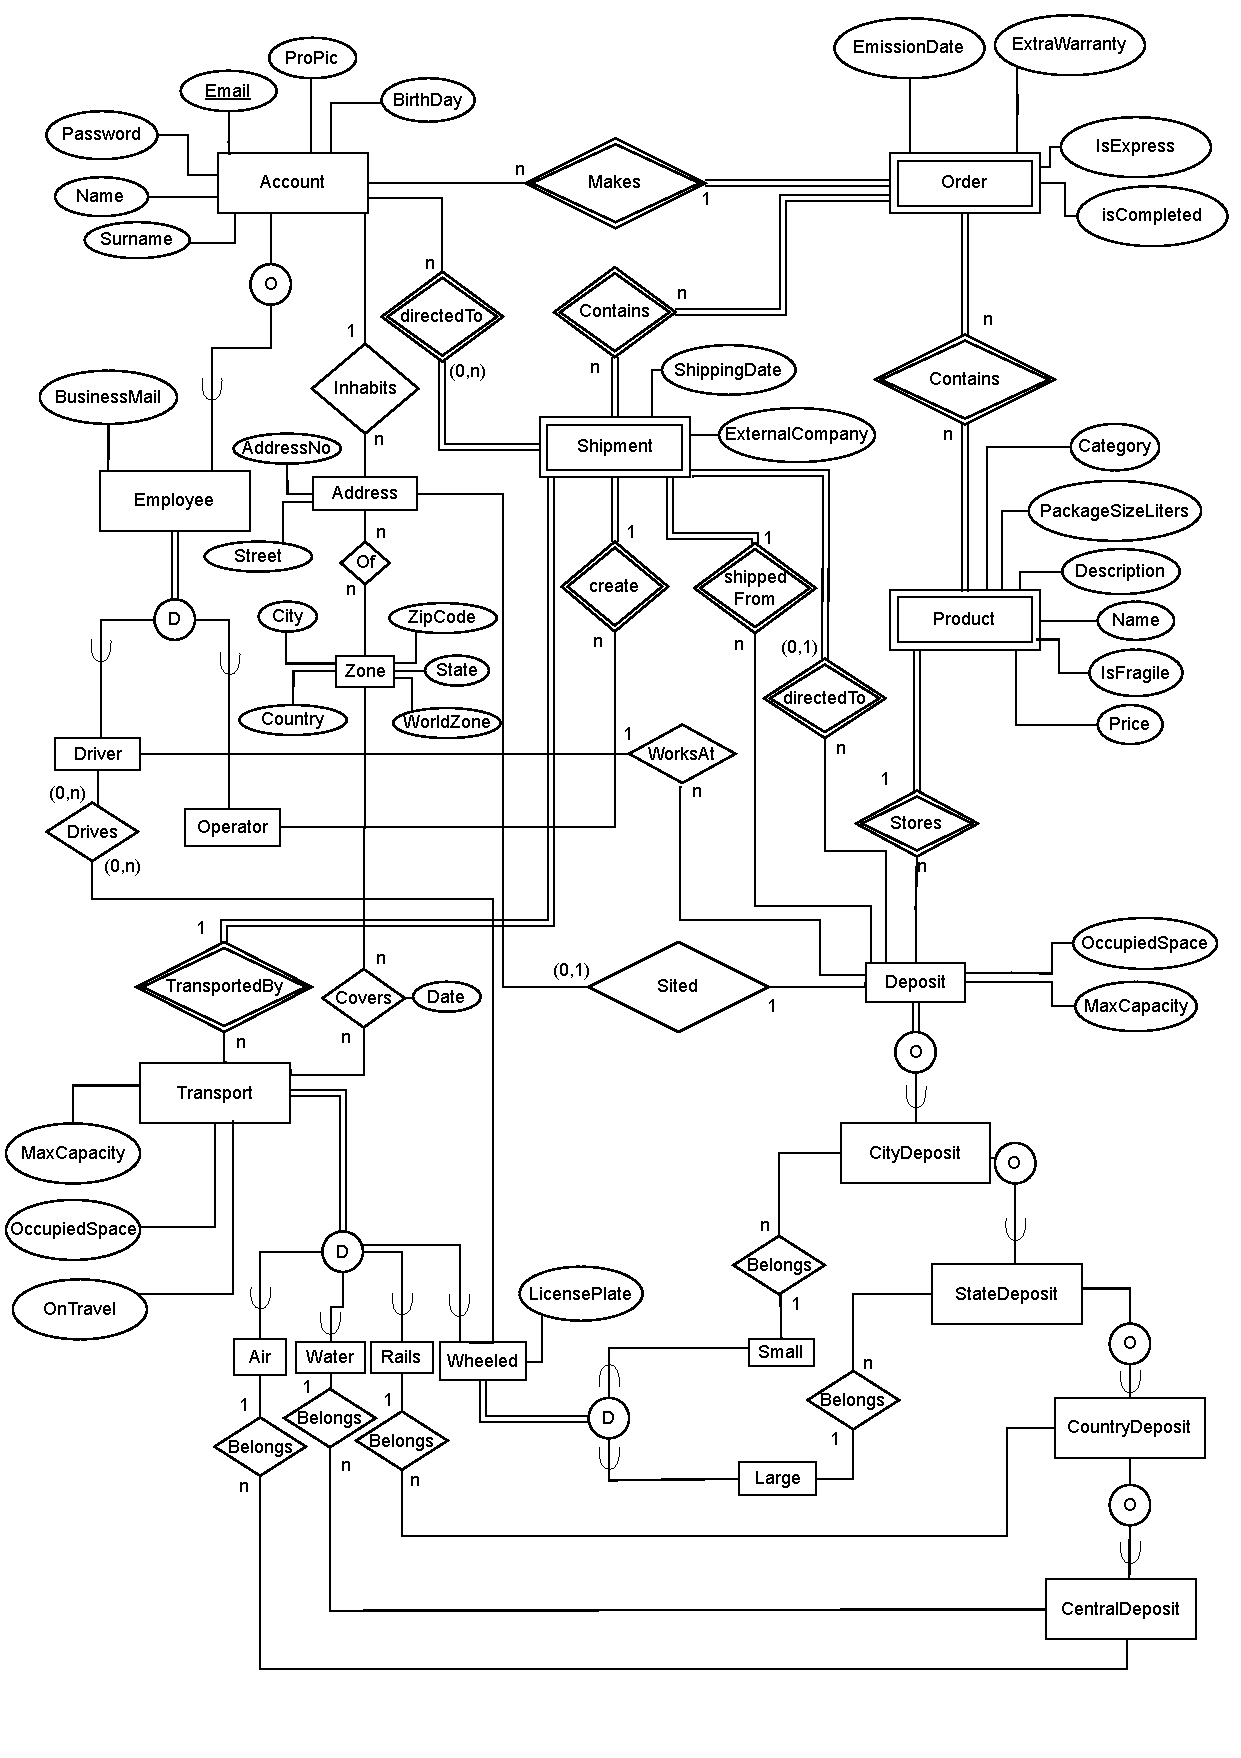
\includegraphics[width=0.9\textwidth]{ER_Diagram.pdf}
\end{center}

% TODO: need to re-export the UML diagram with the new changes. All the changes in the ER diagram are already done in the UML diagram
% If it's needed scale the size of the image with 0.x or 1.x near to \textwidth

\section{UML Class Diagram}
\begin{center}
  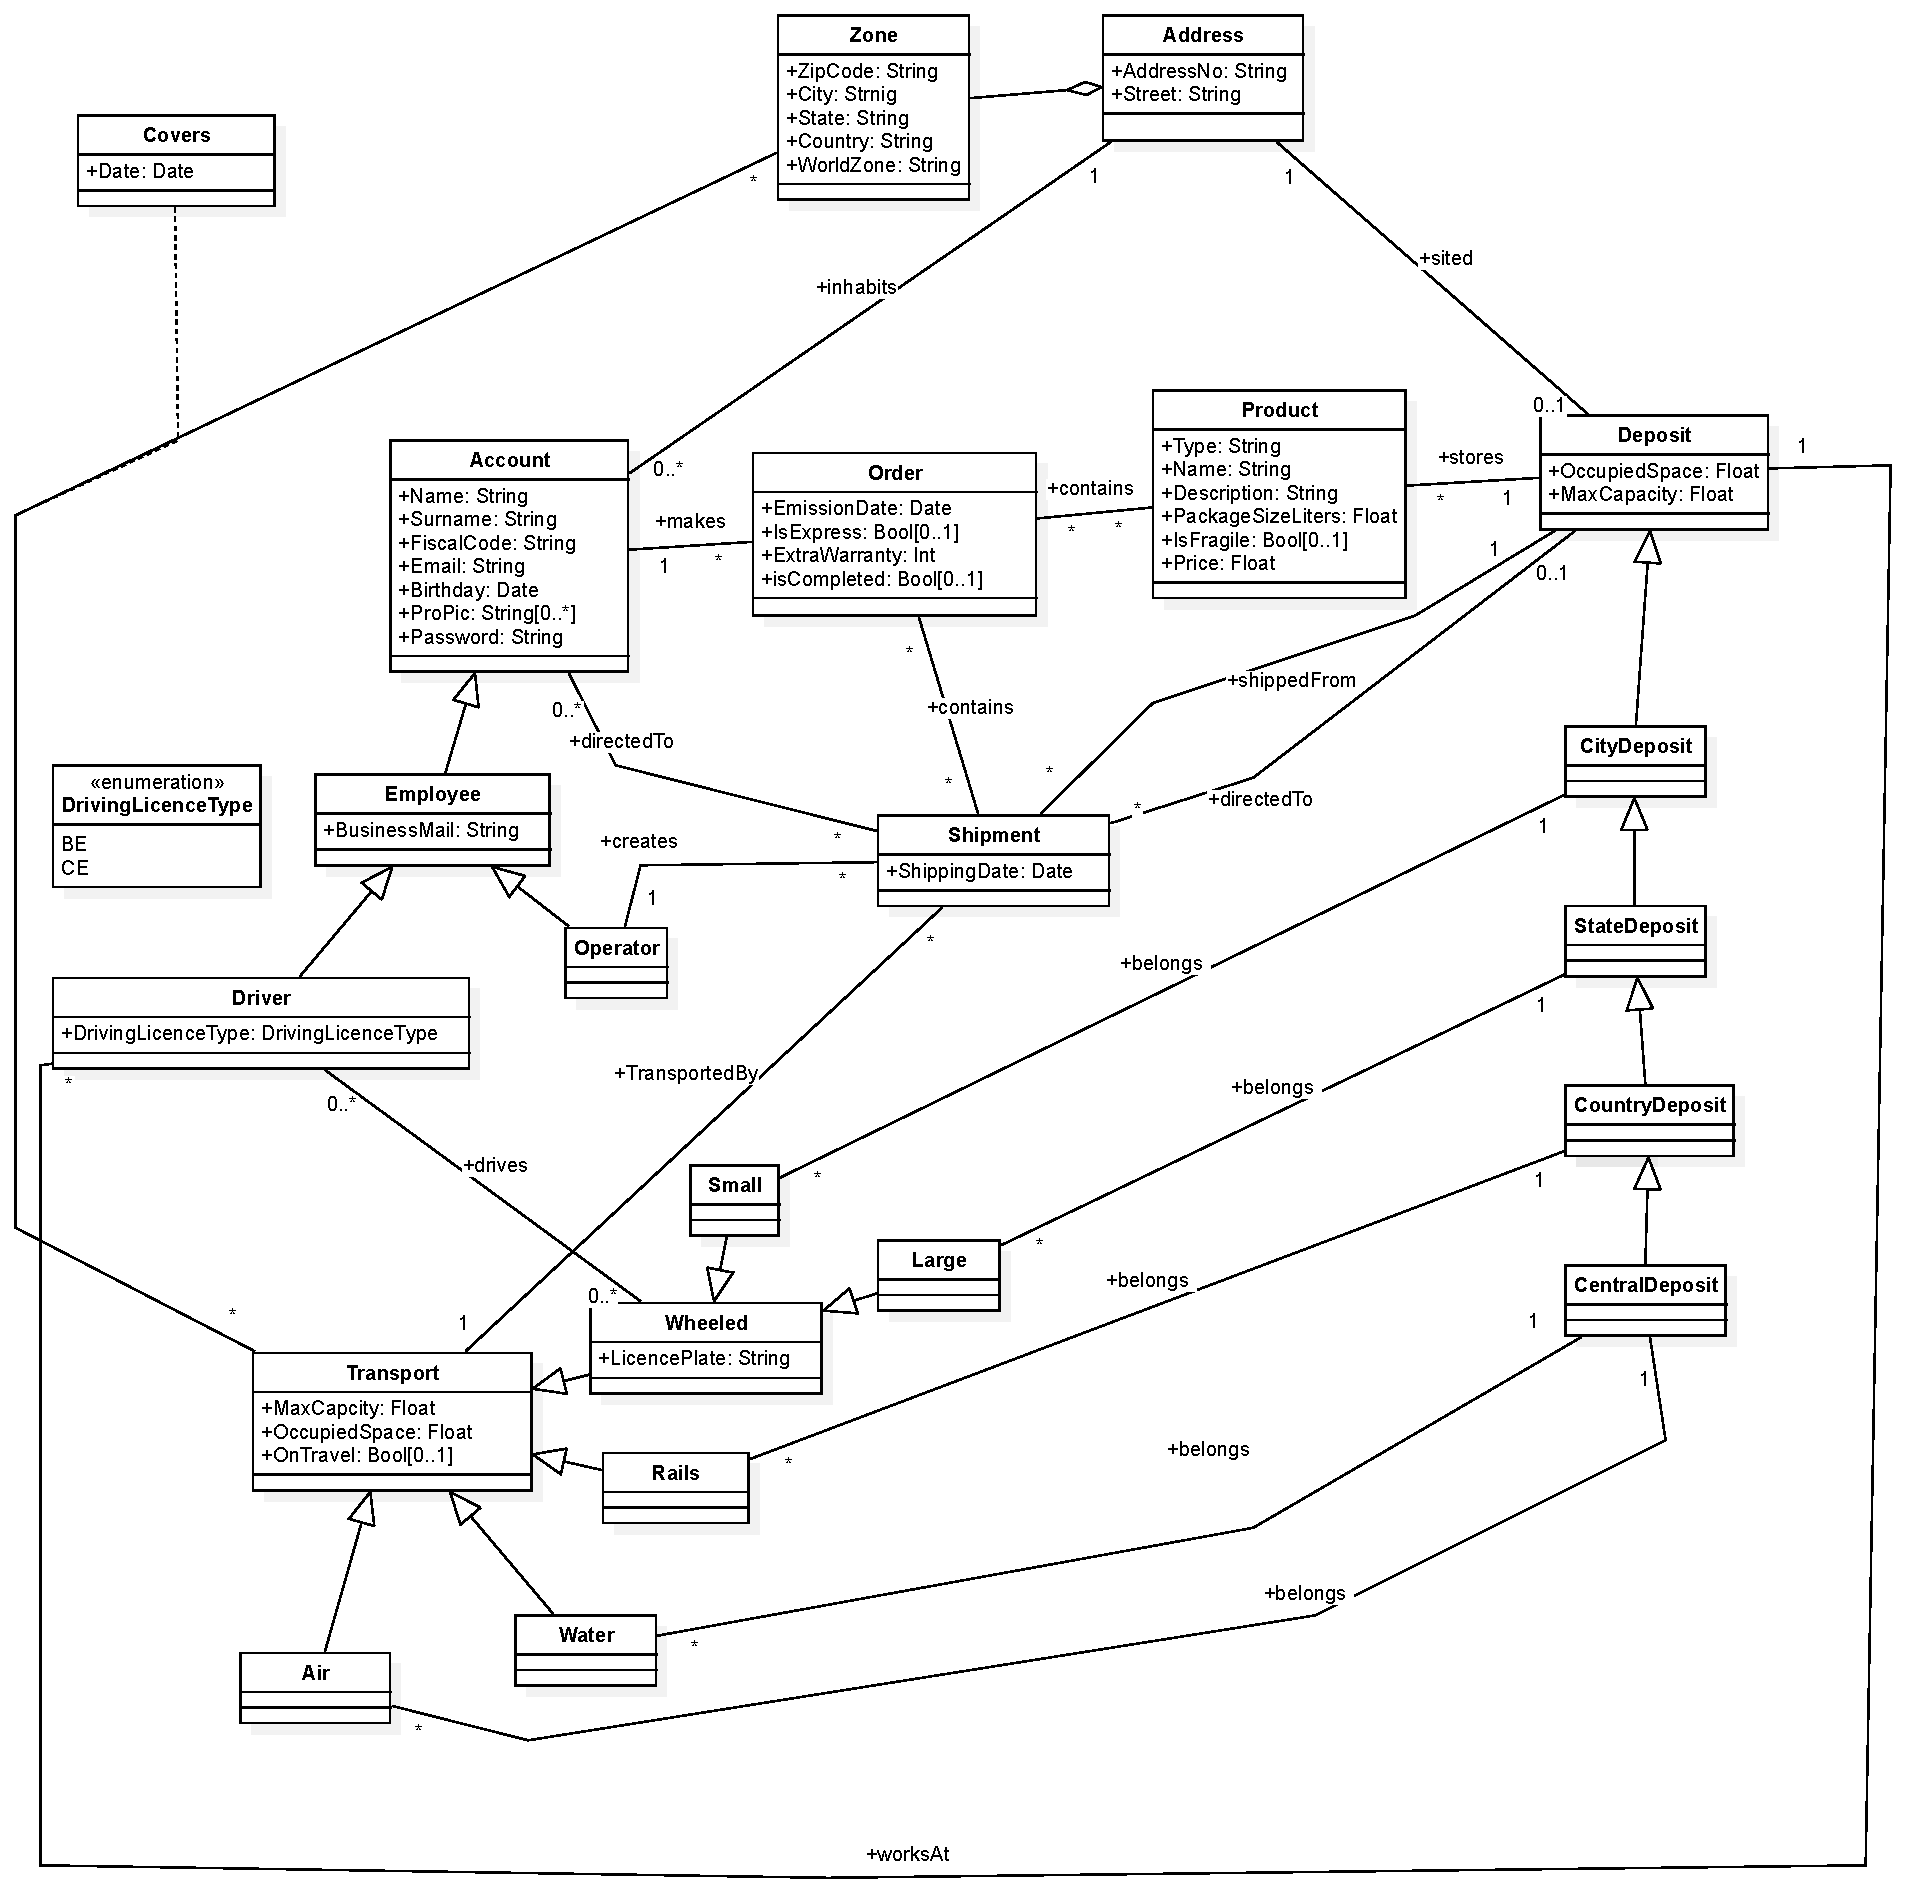
\includegraphics[width=\textwidth]{UML_Class_Diagram.pdf}
\end{center}

\newpage

\section{Ristrutturazione del Diagramma UML}

\subsection{Considerazioni sulla Ristrutturazione}

\subsubsection{Attributi Multipli e Multivalore}

Nello schema concettuale non sono presenti attributi \textbf{Multipli} o \textbf{Multivalore}, in quanto non sono stati ritenuti necessari per la rappresentazione del mini-mondo.

\subsubsection{Attributi Derivati}

Nello schema concettuale sono presenti due attributi \textbf{Derivati}:

\begin{itemize}
  \item L'attributo \textbf{Price} dell'entità \textbf{Shipment}, il quale però non ha necessità di essere conservato, non essendo un attributo di frequente richiesta per il sistema richiesto, e che quindi può essere eventualmente calcolato \textit{on-the-fly} in fase d'interrogazione del database basandosi sugli indirizzi di partenza e arrivo della spedizione e sulle eventuali modalità extra di consegna specificate in \textbf{Order}, come \textit{ExtraWarranty} e \textit{IsExpress}.
  \item L'attributo \textbf{IsCompleted} dell'entità \textbf{Order}, invece, si è scelto di conservarlo, in quanto è un attributo che può essere richiesto frequentemente dal sistema, e richiede un controllo relativamente complesso per essere valorizzato. Un ordine è considerato \textit{completato} se tutti i prodotti che contiene sono stati consegnati all'utente, dunque sarebbe necessario infatti controllare che tutti i prodotti dell'ordine siano stati spediti al destinatario, e che tali spedizioni siano andate a buon fine, coinvolgendo ben quattro entità: \textbf{Order}, \textbf{Product}, \textbf{Shipment} e \textbf{Account}. % * We should add a trigger that does this the first time
  \item L'attributo \textbf{OccupiedSpace} sia dell'entità \textbf{Deposit} che dell'entità \textbf{Transport}, infine, è stato anch'esso conservato, in quanto è un attributo che può essere richiesto frequentemente dal sistema, e richiede un interrogazione con risultato potenzialmente molto grande per essere valorizzata. % * this can be a cool trigger too.
\end{itemize}

\subsubsection{Generalizzazioni e Specializzazioni}

Le varie \textbf{Generalizzazioni} e \textbf{Specializzazioni} presenti nello schema concettuale sono state ristrutturate usando metodologie diverse, in base alla loro natura.

\begin{itemize}
  \item[\textbf{Employee:}] Essendo la specializzazione \textbf{Totale Disgiunta}, ed essendo le classi coinvolte in poche associazioni, si è scelto di accorpare la classe generale in quelle specializzate.
  \item[\textbf{Account:}] Essendo la specializzazione \textbf{Parziale Overlapping}, si è deciso di trasformarla in \textbf{Associazione}, limitando così il più possibile il numero di campi \textbf{NULL} e di \textbf{Vincoli d'Integrità}.
  \item[\textbf{Deposit:}] In questo caso trattandosi di una gerarchia di specializzazione si è scelto di accorpare a cascata le classi specializzate in quella generale, non avendo le classi specializzate attributi ed essendo tutte coinvolte in un'unica associazione concettualmente identica che verrà successivamente analizzata.
  \item[\textbf{Transport:}] Analogamente a quanto visto per \textbf{Deposit}, nonostante non si tratti di una gerarchia, si è scelto di accorpare le classi specializzate in quella generale. 
\end{itemize}

\subsubsection{Analisi delle Ridondanze}\label{Redundancy analysis}

Vediamo infine le ridondanze presenti nello schema concettuale, e come sono state rimosse.

Dalla ristrutturazione delle \textbf{Specializzazioni} di \textbf{Transport} sono emersi quattro attributi che servono essenzialmente lo stesso scopo ma per tipologie diverse di mezzi di trasporto: \textbf{Licence Plate}, \textbf{TrainNo}, \textbf{IMOCode} e \textbf{FlightNo}. Si è quindi deciso di accorpare questi attributi in un unico attributo \textbf{TransportID}, che può essere valorizzato con un identificativo univoco condiviso tra le tipologie di mezzi di trasporto, eliminando la possibilità di valori \textbf{NULL} o di valori uguali per tipi di mezzi diversi che imponevano aggiunta di vincoli o presenza di più attributi.

Inoltre la ristrutturazione delle \textbf{Specializzazioni} di \textbf{Deposit} ha fatto emergere quattro associazioni identiche a meno di vincoli che le riguardano, ovvero le associazioni \textbf{belongs}. È possibile dunque ridurle a un'unica associazione preservando i vincoli.

In ultima analisi, la classe \textbf{Shipment} è coinvolta in due associazioni semanticamente identiche, che si distinguono solo per molteplicità e seconda classe coinvolta, ovvero \textbf{Account} e \textbf{Deposit}. In particolare quella con \textbf{Account} è un'associazione circolare, essendo entrambe le classi associate anche con \textbf{Order}. Si è quindi deciso di eliminare l'associazione con \textbf{Account}, essendo il destinatario della spedizione già noto tramite \textbf{Order}.

\subsection{Identificazione delle Chiavi primarie}

Aldilà delle chiavi primarie già presenti nello schema concettuale esplicitate nel \textbf{diagramma ER} e dell'attributo \textbf{TransportID} introdotto \intlink{Redundancy analysis}{precedentemente}, si è deciso di aggiungere chiavi surrogate per le entità \textbf{Order}, \textbf{Shipment} e \textbf{Deposit}, poiché migrando le chiavi di altre entità si sarebbero ottenute chiavi composte troppo lunghe e complesse.

Per l'entità \textbf{Address} invece, è risultato più appropriato migrare la chiave primaria di \textbf{Zone} essendo una composizione e di conseguenza già concettualmente una \textit{parte} dell'entità \textbf{Address}. 

\newpage

\subsection{Class Diagram Ristrutturato}

% TODO: @zGenny review restructured diagram, if it's ok export it and uncommend this part. To adjust size add 0.x or 1.x near to \textwidth

% \begin{center}
  % ! USE THE NAME MENTIONED HERE FOR THE FILE
%   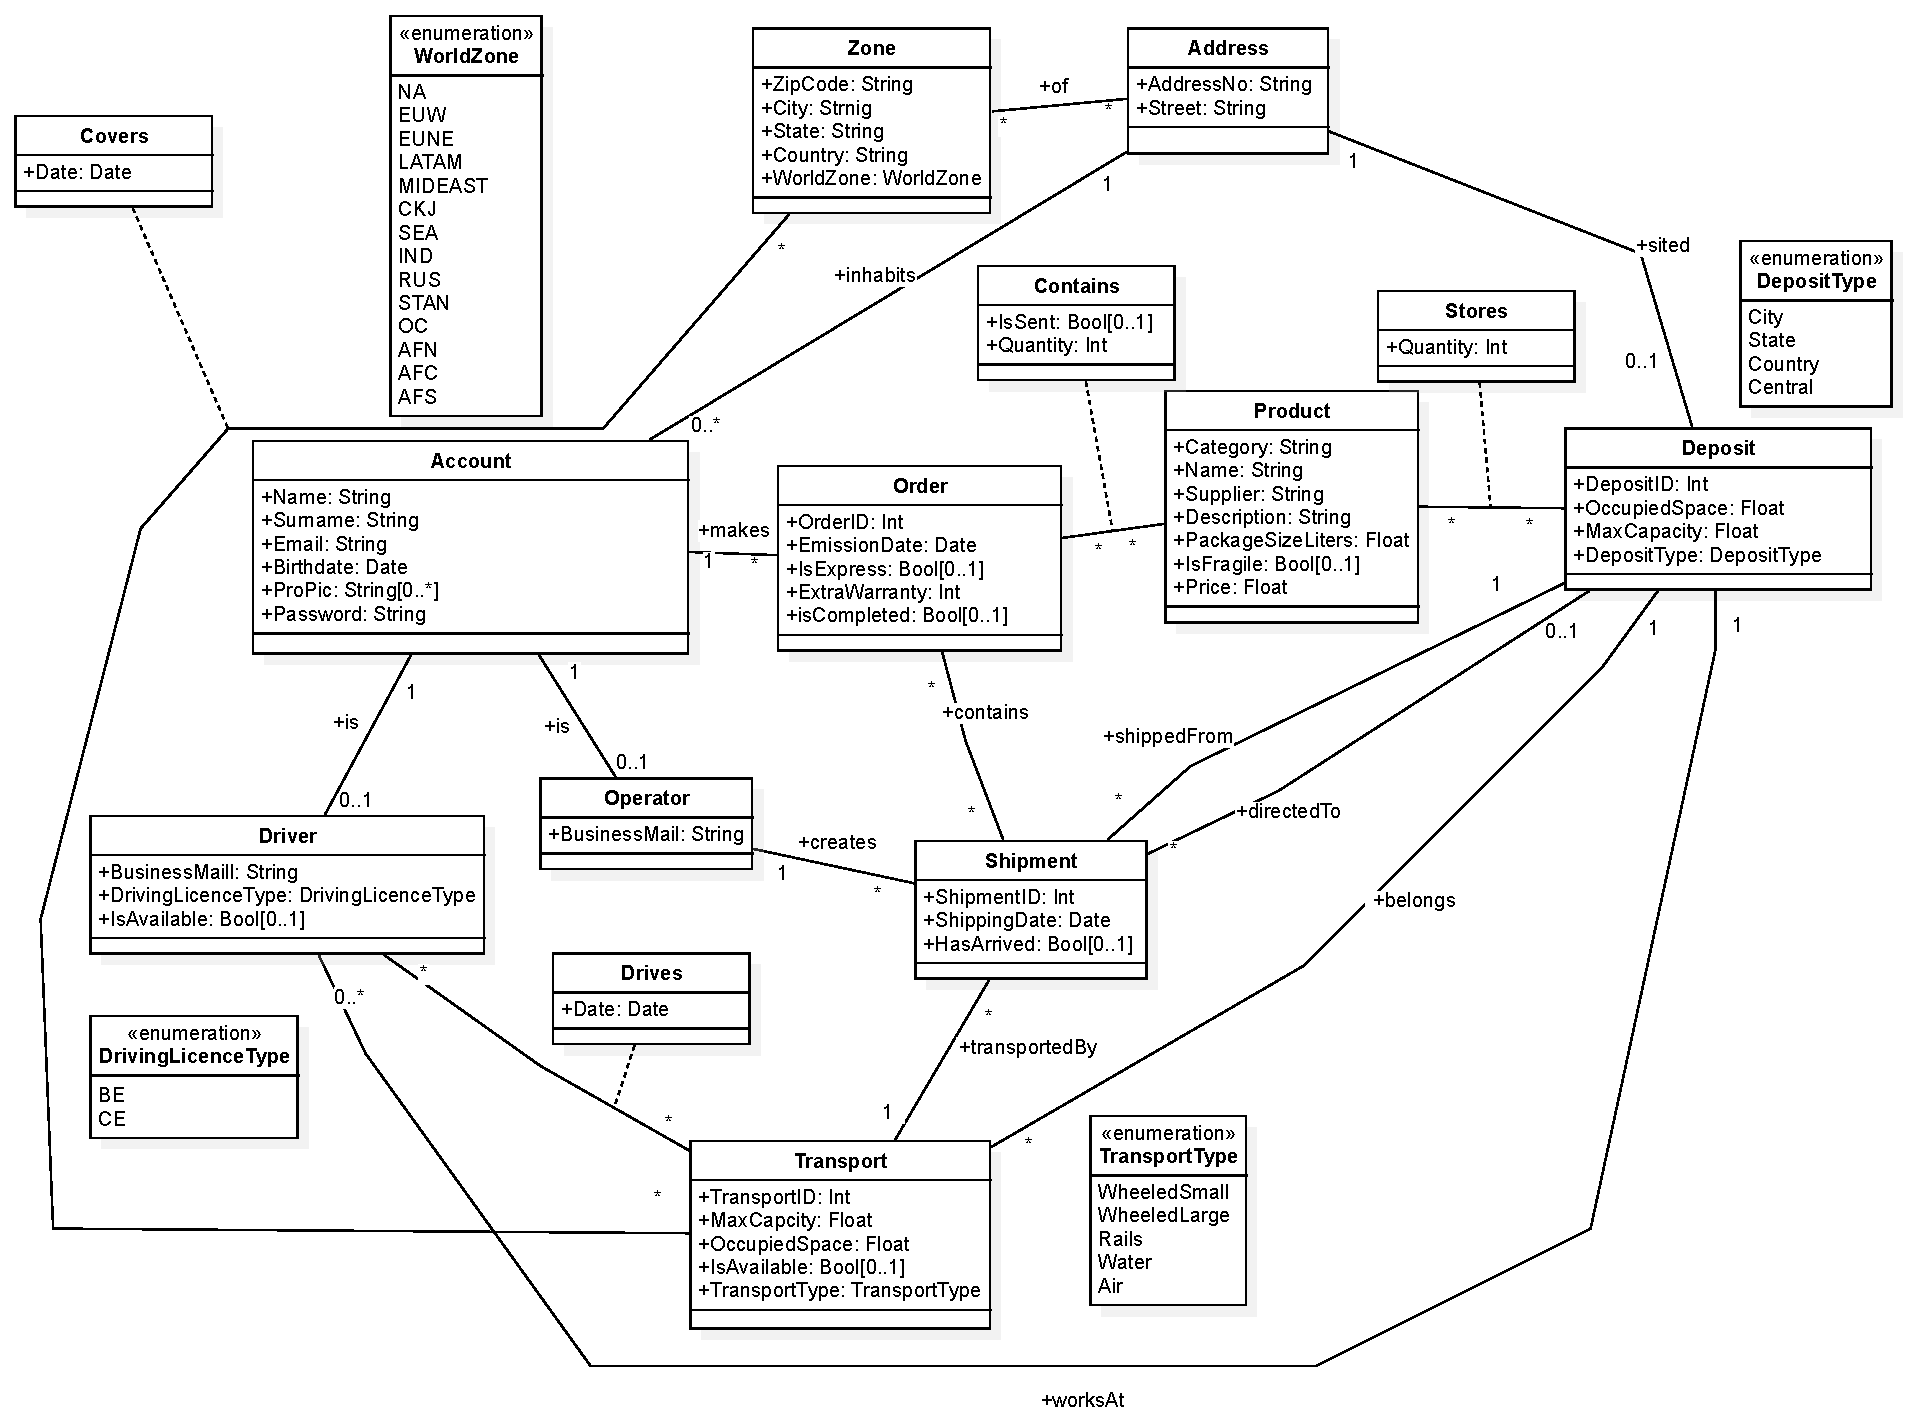
\includegraphics[width=\textwidth]{UML_Class_Diagram_Restructured.pdf} 
% \end{center}

\newpage

\section{Dizionari}

\subsection{Dizionario delle Classi}

\customTable{cYY}[Dizionario delle classi Prima Parte]{\textbfB{Classe} & \textbfB{Descrizione} & \textbfB{Attributi}}{
  \textbf{Account} & Generico utente che utilizza il sistema per effettuare ordini. & 
  {\footnotesize 
  \textbf{Name:} (\textit{string}): Nome dell'utente;
  
  \textbf{Surname} (\textit{string}): Cognome dell'utente;
  
  \textbf{Email} (\textit{string}): Chiave Primaria. Email dell'utente;

  \textbf{Birthdate} (\textit{date}): Data di nascita dell'utente;

  \textbf{ProPic} (\textit{string}): Eventuale immagine profilo dell'utente;

  \textbf{Password} (\textit{string}): Password dell'utente;  
  }\\


  \textbf{Operator} & Account di un impiegato che si occupa di creare le spedizioni. &
  {\footnotesize
  \textbf{BusinessMail} (\textit{string}): Chiave Primaria. Email aziendale dell'operatore;
  }\\


  \textbf{Driver} & Account di un autista che si occupa di effettuare le consegne. &
  {\footnotesize
  \textbf{BusinessMail} (\textit{string}): Chiave Primaria. Email aziendale dell'autista;

  \textbf{DrivingLincenceType} (\textit{DrivingLincenceType}): Tipologia di patente dell'autista;

  \textbf{IsAvailable} (\textit{bool}): Indica se l'autista è disponibile o meno;
  }\\


  \textbf{Order} & Ordine effettuato da un utente. Può contenere più prodotti e può essere spedito in più spedizioni. &
  {\footnotesize
  \textbf{OrderID} (\textit{integer}): Chiave Surrogata. Identificativo dell'ordine;

  \textbf{EmissionDate} (\textit{date}): Data di emissione dell'ordine;

  \textbf{IsExpress} (\textit{bool}): Indica se l'ordine è espresso o meno;

  \textbf{ExtraWarranty} (\textit{bool}): Indica se è stata acquistata una garanzia extra o meno;

  \textbf{IsCompleted} (\textit{bool}): Indica se l'ordine è stato completato o meno;
  }\\


  \textbf{Shipment} & Singola spedizione partita da un deposito. Può contenere più ordini e può raggiungere a più utenti o a un deposito. &
  {\footnotesize
  \textbf{ShipmentID} (\textit{integer}): Chiave Surrogata. Identificativo della spedizione; 

  \textbf{ShippingDate} (\textit{date}): Data della spedizione;
  }\\  
}

\newpage

\customTable{cYY}[Dizionario delle classi Seconda Parte]{\textbfB{Classe} & \textbfB{Descrizione} & \textbfB{Attributi}}{
  \textbf{Product} & Prodotto acquistabile da un utente. Può essere conservato in più depositi. &
  { \footnotesize
    \textbf{Type} (\textit{string}): Categoria del prodotto;

    \textbf{Name} (\textit{string}): Chiave Primaria. Nome del prodotto;

    \textbf{Supplier} (\textit{string}): Chiave Primaria. Fornitore del prodotto. Di default è \textit{UninaDelivery};
  
    \textbf{Description} (\textit{string}): Descrizione del prodotto;

    \textbf{PackageSizeLiters} (\textit{float}): Dimensione del prodotto in litri;

    \textbf{IsFagile} (\textit{bool}): Indica se il prodotto è fragile o meno;

    \textbf{Price} (\textit{float}): Prezzo del prodotto;
  }\\


  \textbf{Deposit} & Deposito per la conservazione di prodotti. Può contenere più prodotti e può essere raggiunto da più spedizioni. &
  {\footnotesize
  \textbf{DepositID} (\textit{integer}): Chiave Surrogata. Identificativo del deposito;

  \textbf{OccupiedSpace} (\textit{float}): Spazio del deposito attualmente occupato;

  \textbf{MaxCapacity} (\textit{float}): Spazio massimo del deposito;

  \textbf{DepositType} (\textit{DepositType}): Tipologia del deposito;
  }\\
  

  \textbf{Zone} & Zona del mondo raggiungibile da un mezzo di trasporto. Contiene più indirizzi. &
  {\footnotesize
  \textbf{ZipCode} (\textit{string}): Chiave Primaria. Codice di Avviamento Postale della zona;

  \textbf{City} (\textit{string}): Città in cui si trova la zona;

  \textbf{Country} (\textit{string}): Chiave Primaria. Paese in cui si trova la zona;
  
  \textbf{WorldZone} (\textit{string}): Zona del mondo in cui si trova la zona;
  }\\

  \textbf{Address} & Indirizzo di un utente o di un deposito. & 
  {\footnotesize

  \textbf{AddressNo} (\textit{string}): Chiave Primaria. Numero civico dell'indirizzo; 

  \textbf{Street} (\textit{string}): Via dell'indirizzo;
  }\\

  \textbf{Transport} & Mezzo di trasporto utilizzato per le spedizioni. & 
  {\footnotesize
  \textbf{TransportID} (\textit{integer}): Chiave Surrogata. Identificativo del mezzo di trasporto;

  \textbf{MaxCapacity} (\textit{float}): Capacità massima del mezzo di trasporto;

  \textbf{OccupiedSpace} (\textit{float}): Spazio attualmente occupato dal mezzo di trasporto;

  \textbf{IsAvailable} (\textit{bool}): Indica se il mezzo di trasporto è disponibile o meno. Il campo sarà valorizzato a \textit{true} solo se il mezzo non è già in viaggio;
  
  \textbf{TransportType} (\textit{TransportType}): Tipologia del mezzo di trasporto;
  }\\

}

\newpage
\subsection{Dizionario delle Associazioni}

\customTable{cYYY}[Dizionario delle associazioni Prima Parte]{\textbfB{Associazione} & \textbfB{Descrizione} & \textbfB{Attributi} & \textbfB{Classi Coinvolte}}{
  Val 1 & Val 2 & Val 3 & Val 4 \\
  Val 1.2 & Val 2.2 & Val 3.2 & Val 4.2 \\
}
  

\newpage
\subsection{Dizionario dei Vincoli}

\customTable{ccY}[Dizionario dei vincoli Prima Parte]{\textbfB{Vincolo} & \textbfB{Tipologia} & \textbfB{Descrizione}}{
  Val 1 & Val 2 & Val 3 \\
  Val 1.2 & Val 2.2 & Val 3.2 \\
}




% TODO: @RiccardoElena @zGenny write this section
  % it should contains:
  % [x] all the considerations about the UML diagram
  % [x] the changes made to the UML diagram
  % [ ] the new UML diagram
  % [ ] constrints dictonary (table (?)). Styled as the example in the slides

  % Chapter 3 - "Schema Logico"
  \chapter{Schema Logico}

\section{Traduzione delle Associazioni}

\customTable{cY}[Dizionario delle classi Seconda Parte]{\textbfB{Associazione} & \textbfB{Strategia di Traduzione}}{
  \textbf{makes} & {\footnotesize Migrazione della \underline{chiave primaria} di \textbf{Account} in \textbf{Order}.} \\
  \textbf{contains} & {\footnotesize Migrazione della \underline{chiave primaria} di \textbf{Product} in \textbf{Order}.} \\
  \textbf{stores} & {\footnotesize Definizione di una nuova tabella \textbf{Stores} con chiavi esterne verso \textbf{Product} e \textbf{Deposit}, oltre che gli attributi della relazione.} \\
  \textbf{worksAt} & {\footnotesize Migrazione della \underline{chiave primaria} di \textbf{Deposit} in \textbf{Driver}.} \\
  \textbf{belongs} & {\footnotesize Migrazione della \underline{chiave primaria} di \textbf{Deposit} in \textbf{Transport}.} \\
  \textbf{drives} & {\footnotesize Definizione di una nuova tabella \textbf{Drives} con chiavi esterne verso \textbf{Transport} e \textbf{Driver}, oltre che gli attributi della relazione.} \\
  \textbf{transportedBy} & {\footnotesize Migrazione della \underline{chiave primaria} di \textbf{Transport} in \textbf{Shipment}.} \\
  \textbf{covers} & {\footnotesize Definizione di una nuova tabella \textbf{Covers} con chiavi esterne verso \textbf{Transport} e \textbf{Area}, oltre che gli attributi della relazione.} \\
  \textbf{ships} & {\footnotesize Definizione di una nuova tabella \textbf{Ships} con chiavi esterne verso \textbf{Shipment} e \textbf{Order}.} \\
  \textbf{shippedFrom} & {\footnotesize Migrazione della \underline{chiave primaria} di \textbf{Deposit} in \textbf{Shipment}.} \\
  \textbf{shippedTo} & {\footnotesize Migrazione della \underline{chiave primaria} di \textbf{Deposit} in \textbf{Shipment}.} \\
  \textbf{is} & {\footnotesize Migrazione della \underline{chiave primaria} di \textbf{Account} in \textbf{Operator}.} \\
  \textbf{is} & {\footnotesize Migrazione della \underline{chiave primaria} di \textbf{Account} in \textbf{Driver}.} \\
  \textbf{inhabits} & {\footnotesize Migrazione della \underline{chiave primaria} di \textbf{Address} in \textbf{Account}.} \\
  \textbf{sited} & {\footnotesize Accorpamento delle classi coinvolte nella classe \textbf{Deposit}.}\\
  \textbf{located} & {\footnotesize Migrazione della \underline{chiave primaria} di \textbf{Address} in \textbf{Area}.} \\
}

\section{Traduzione delle Classi}

\subsection{Considerazioni sulla Traduzione delle Classi}

Per quanto riguarda l'individuazione delle chiavi primarie, ciò è stato già fatto nella sezione \intlink{individuazioneDelleChiaviPrimarie}{identificazione delle chiavi primarie}.

Dalla \textbf{traduzione delle associazioni} si è evidenziato come, per via delle strategie utilizzate per la traduzione, la classe \textbf{Address} sia ridondante. Infatti la classe \textbf{Deposit} e la classe \textbf{Account} ne contengono tutti i campi, essendo tutti chiavi primarie, e per la classe \textbf{Area} la migrazione delle chiavi avveniva \textit{verso \textbf{Address}}, diventando anch'esse chiavi primarie e venendo ereditate da \textbf{Deposit} e \textbf{Account}.
È sufficiente quindi per eliminare la classe \textbf{Address} oltre alle strategie già messe in atto durante la \textbf{traduzione delle associazioni} migrare le chiavi primarie di \textbf{Area} direttamente verso \textbf{Deposit} e \textbf{Account}, andando a diminuire l'overhead e risolvendo in automatico vincoli come \intlink{isAddressForSomethingGeneral}{\textbf{isAddressForSomethingGeneral}}.

Per mantenere la consistenza del database, va anche introdotto un vincolo di unicità nella nuova classe accorpata \textbf{Deposit}. Per garantire l'associazione di tipo \(1:1\) tra \textbf{Deposit} e \textbf{Address} è necessario che la quadrupla di campi \textit{AddressNo}, \textit{Street}, \textit{ZipCode} e \textit{Country} sia unica nella tabella.
\section{Schema Logico}

\begin{note}[Indicazioni di Chiave Primaria e Chiave Esterna]
  Per evidenziare la presenza di \textbf{chiavi primarie} e \textbf{chiavi esterne} nei diagrammi, si è deciso sottolineare le \underline{chiavi primarie} e mettere in corsivo le \textit{chiavi esterne}.

  Per evitare superflue verbosità si è scelto di chiamare tutti i campi che rappresentano una chiave esterna con il nome della chiave primaria cui fanno riferimento. In caso di ambiguità, si è scelto di utilizzare il nome dell'associazione tradotta con l'uso di tale chiave o la classe a cui appartiene la chiave primaria a cui fa riferimento la chiave esterna.
\end{note}


\customTableLogic{|Y|Y|Y|Y|Y|}{5}{Area}{
  \underline{ZipCode} & City & State & \underline{Country} & WorldZone
}

\customTableLogic{|Y|Y|Y|Y|Y|}{5}{Account}{
  Name & Surname & \underline{Email} & Birthdate & ProPic \\
  \hline
  Password & \textit{AddressNo} & \textit{Street} & \textit{ZipCode} & \textit{Country}
}
% TODO: @zGenny 
\customTableLogic{|Y|Y|Y|Y|Y|}{5}{Order}{
  \underline{OrderID} & EmissionDate & isExpress & ExtraWarranty & IsCompleted \\
  \hline
  \textit{Email} & \textit{Quantity} & \textit{Name} & \textit{Supplier} & - 
}

\customTableLogic{|Y|Y|Y|Y|}{4}{Product}{
  Category & \underline{Name} & \underline{Supplier} & Description \\
  \hline
  PackageSizeLiters & isFragile & Price & ---
}

\customTableLogic{|Y|Y|Y|Y|}{4}{Stores}{
  \textit{Name} & \textit{Supplier} & \textit{DepositID} & Quantity
}

\customTableLogic{|Y|Y|Y|Y|}{4}{Deposit}{
  \underline{DepositID} & OccupiedSpace & MaxCapacity & DepositType \\
  \hline
  \textit{AddressNo} & \textit{Street} & \textit{ZipCode} & \textit{Country}
}

\customTableLogic{|Y|Y|Y|Y|}{4}{Shipment}{
  \underline{ShipmentID} & ShippingDate & HasArrived & \textit{ShippedFrom} \\
  \hline
  \textit{DirectedTo} & \textit{BusinessMail} & \textit{TransportID} & ---
}

\customTableLogic{|Y|Y|}{2}{Ships}{
  \textit{ShipmentID} & \textit{OrderID}
}

\customTableLogic{|Y|Y|}{2}{Operator}{
  \underline{BusinessMail} & \textit{Email}
}

\customTableLogic{|Y|Y|Y|}{3}{Transport}{
  \underline{TransportID} & MaxCapacity & OccupiedSpace \\
  \hline IsAvailable & TransportType & \textit{DepositID}
}

\customTableLogic{|Y|Y|Y|}{3}{Drives}{
  \textit{TransportID} & \textit{BusinessMail} & Date
}

\customTableLogic{|Y|Y|Y|}{3}{Driver}{
  \underline{BusinessMail} & DrivingLincenceType & IsAvailable \\
  \hline
  \textit{Email} & \textit{DepositID} & ---
}

\customTableLogic{|Y|Y|Y|Y|}{4}{Covers}{
  \textit{TransportID} & \textit{ZipCode} & \textit{Country} & Date
}


   % Chapter 4 - "Implementazione delle Tabelle"
   \chapter{Implementazione delle Tabelle}

In conclusione si riportano le istruzioni per l'implementazione fisica del database.

Come DBMS provider si è scelto di utilizzare PostgreSQL, per la sua facilità di utilizzo e la sua affidabilità.

Il database è hostato localmente per rendere più agevole la connessione.

Per pulizia del codice si è preferito lavorare su uno \textbf{schema} creato appositamente per il progetto, chiamato \textbf{UninaDelivery}.

\section{Definizione dei Domini Personalizzati}

Vista la vasta gamma di vincoli di dominio simili su vari campi, si è deciso di definire dei domini personalizzati per facilitare la creazione delle tabelle.

\begin{lstlisting}
  CREATE DOMAIN letterString AS text CHECK (VALUE ~ '^[a-zA-Z]+$');
  
  CREATE DOMAIN numericString AS text CHECK (VALUE ~ '^[0-9]+$');
  
  CREATE DOMAIN alphanumericString AS text CHECK (VALUE ~ '^\w+[\w\s.]$');
  
  CREATE DOMAIN emailString AS text CHECK (
    VALUE ~ '^\w+[\w.]*\w@[a-zA-Z.]+\.[a-zA-Z]{2,}$'
  );
\end{lstlisting}

Inoltre per i campi che nel diagramma ristrutturato sono stati definiti come \textbf{enumerazioni}, si è deciso di utilizzare dei tipi enumerati personalizzati.

\begin{lstlisting}
  CREATE TYPE WorldZone AS ENUM (
    'NA', 'EUW', 'EUNE', 'LATAM', 'MIDEAST', 'CKJ', 'SEA', 'IND', 'RUS', 'STAN', 
    'OC', 'AFN', 'AFC', 'AFS'
  );

  CREATE TYPE DepositType AS ENUM (
    'City', 'State', 'Country', 'Central'
  );

  CREATE TYPE TransportType AS ENUM (
    'WheeledSmall', 'WheeledLarge', 'Rails', 'Water', 'Air'
  );
  
  CREATE TYPE DrivingLicenceType AS ENUM ('BE', 'CE');
\end{lstlisting}

\section{Creazione delle Tabelle}

Vediamo ora la creazione delle tabelle, con annessi vincoli di dominio e di n-upla, oltre che le chiavi primarie e le chiavi esterne.

\begin{lstlisting}[caption={Creazione della tabella \textbf{Area}}]
  CREATE TABLE Area (
    ZipCode numericString NOT NULL,
    City letterString NOT NULL,
    State letterString NOT NULL,
    Country letterString NOT NULL,
    WorldZone WorldZone NOT NULL
  );
  ALTER TABLE Area ADD CONSTRAINT Area_pk PRIMARY KEY (ZipCode, Country);
\end{lstlisting}

\begin{lstlisting}[caption={Creazione della tabella \textbf{Account}}]
  CREATE TABLE Account (
    Name letterString NOT NULL,
    Surname letterString NOT NULL,
    Email emailString NOT NULL,
    Birthdate date NOT NULL,
    ProPic text,
    Password text NOT NULL,
    AddressNo alphNumString NOT NULL,
    Street alphNumString NOT NULL,
    ZipCode numericString NOT NULL,
    Country letterString NOT NULL
  );
  ALTER TABLE account ADD CONSTRAINT Account_pk PRIMARY KEY (Email);
  ALTER TABLE account ADD CONSTRAINT validAccountBirthdate CHECK (
    EXTRACT( YEAR FROM age(Birthdate)) >= 16 
  );
  ALTER TABLE account ADD CONSTRAINT formatAccountPassword CHECK(
    Password ~ '^[A-Fa-f0-9]{64}$'
  );
  ALTER TABLE account ADD CONSTRAINT formatAccountProPic CHECK (
    ProPic ~ '^\/9j\/4AAQSkZJRg[-A-Za-z0-9+\/]*={0,2}$'
  );
  ALTER TABLE Account ADD CONSTRAINT formatAccountAddressNo CHECK (
    AddressNo ~ '^[1-9]\d*[a-z]?(?:BIS)?$'
  );
  ALTER TABLE Account ADD CONSTRAINT account_fk FOREIGN KEY (ZipCode, Country) REFERENCES Area(ZipCode, Country) ON DELETE CASCADE ON UPDATE CASCADE;
\end{lstlisting}
  

\newpage
\begin{lstlisting}[caption={Creazione della tabella \textbf{Order}}]
  CREATE TABLE "Order"(
    OrderID SERIAL, 
    EmissionDate Date NOT NULL,
    IsExpress boolean,
    ExtraWarranty smallint NOT NULL,
    IsCompleted boolean,
    Email emailString,
    Quantity integer NOT NULL
  );
  ALTER TABLE "Order" ADD CONSTRAINT Order_pk PRIMARY KEY (OrderID);
  ALTER TABLE "Order" ADD CONSTRAINT formatOrderExtraWarranty CHECK (
    ExtraWarranty >=0
  );
  ALTER TABLE "Order" ADD CONSTRAINT Order_fk FOREIGN KEY (Email) REFERENCES Account(Email) ON DELETE SET NULL ON UPDATE CASCADE;
  ALTER TABLE "Order" ADD CONSTRAINT formatOrderEmissionDate CHECK (
    EmissionDate <= current_date
  );
  ALTER TABLE "Order" ADD CONSTRAINT formatOrderQuantity CHECK (
    Quantity > 0
  );
\end{lstlisting}

\begin{lstlisting}[caption={Creazione della tabella \textbf{Stores}}]
  CREATE TABLE Stores(
    Name text NOT NULL,
    Supplier text NOT NULL,
    DepositID integer NOT NULL,
    Quantity integer NOT NULL
  );
  ALTER TABLE Stores ADD CONSTRAINT noDuplicateProductInDeposit UNIQUE (Name, Supplier, DepositID);
  ALTER TABLE Stores ADD CONSTRAINT Stores_fk_Product FOREIGN KEY (Name, Supplier) REFERENCES Product(Name, Supplier) ON DELETE CASCADE ON UPDATE CASCADE;
  ALTER TABLE Stores ADD CONSTRAINT Stores_fk_Deposit FOREIGN KEY (DepositID) REFERENCES Deposit(DepositID) ON DELETE CASCADE ON UPDATE CASCADE;
  ALTER TABLE Stores ADD CONSTRAINT formatStoresQuantity CHECK(Quantity > 0);
\end{lstlisting}

\newpage

\begin{lstlisting}[caption={Creazione della tabella \textbf{Deposit}}]
  CREATE TABLE Deposit (
    DepositID SERIAL NOT NULL,
    OccupiedSpace real NOT NULL DEFAULT 0,
    MaxCapacity real NOT NULL,
    DepositType DepositType NOT NULL,
    AddressNo alphNumString NOT NULL,
    Street alphNumString NOT NULL,
    ZipCode numericString NOT NULL,
    Country letterString NOT NULL
  );
  ALTER TABLE Deposit ADD CONSTRAINT Deposit_pk PRIMARY KEY ( DepositID);
  ALTER TABLE Deposit ADD CONSTRAINT foramtDepositOccupiedSpace CHECK(
    OccupiedSpace >= 0
  );
  ALTER TABLE Deposit ADD CONSTRAINT foramtDepositMaxCapacity CHECK(
    MaxCapacity > 0
  );
  ALTER TABLE Deposit ADD CONSTRAINT checkDepositFullness CHECK (
    OccupiedSpace <= MaxCapacity
  );
  ALTER TABLE Deposit ADD CONSTRAINT formatDepositAddressNo CHECK (
    AddressNo ~ '^[1-9]\d*[a-z]?(?:BIS)?$'
  );
  ALTER TABLE Deposit ADD CONSTRAINT Deposit_fk FOREIGN KEY (ZipCode, Country) REFERENCES Area(ZipCode, Country) ON DELETE CASCADE ON UPDATE CASCADE;
  ALTER TABLE deposit ADD CONSTRAINT onlyOneDepositPerAddress UNIQUE(AddressNo, Street, ZipCode, Country);
\end{lstlisting}

\newpage

\begin{lstlisting}[caption={Creazione della tabella \textbf{Product}}]
  CREATE TABLE Product (
    Category letterString NOT NULL,
    Name text NOT NULL,
    Supplier text NOT NULL,
    Description text NOT NULL,
    PackageSizeLiters real NOT NULL,
    IsFragile boolean,
    Price numeric(100,2)
  );
  ALTER TABLE Product ADD CONSTRAINT Product_pk PRIMARY KEY (Name,Supplier);
  ALTER TABLE Product ADD CONSTRAINT formatProductName CHECK(
    Name ~ '^[a-zA-Z0-9]+[\ a-zA-Z0-9!@#$%^&*()_+{}\[\]:;<>,.?''~\\\/-]*$'
  );
  ALTER TABLE Product ADD CONSTRAINT formatProductDescription CHECK(
    Description ~ '^[a-zA-Z0-9]+[\ a-zA-Z0-9!@#$%^&*()_+{}\[\]:;<>,.?''~\\\/-]*$'
  );
  ALTER TABLE Product ADD CONSTRAINT formatProductSupplier CHECK(
    Supplier ~ '^[a-zA-Z0-9]+[\ a-zA-Z0-9!@#$%^&*()_+{}\[\]:;<>,.?''~\\\/-]*$'
  );
  ALTER TABLE Product ADD CONSTRAINT formatProductPackageSizeLiters CHECK(
    PackageSizeLiters > 0
  );
  ALTER TABLE Product ADD CONSTRAINT formatProductPrice CHECK(
    Price > 0
  );
  ALTER TABLE Product ADD CONSTRAINT checkProductDescriptionOnTopic CHECK(
    (Description ILIKE ('% ' || Name || '%')) AND 
    (Description ILIKE ('% ' || Supplier || '%'))
  )
\end{lstlisting}

\begin{lstlisting}[caption={Creazione della tabella \textbf{Covers}}]
  CREATE TABLE Covers (
    TransportID integer NOT NULL,
    ZipCode numericString NOT NULL,
    Country letterString NOT NULL,
    Date date NOT NULL,
    OccupiedSpace real NOT NULL DEFAULT 0
  );
  ALTER TABLE Covers ADD CONSTRAINT Covers_fk_Transport FOREIGN KEY (TransportID) REFERENCES Transport(TransportID) ON DELETE CASCADE ON UPDATE CASCADE;
  ALTER TABLE Covers ADD CONSTRAINT Covers_fk_Area FOREIGN KEY (ZipCode, Country) REFERENCES Area(ZipCode, Country) ON DELETE CASCADE ON UPDATE CASCADE;
  ALTER TABLE Covers ADD CONSTRAINT onlyOneAreaPerDay UNIQUE (TransportID, Date);
  ALTER TABLE Covers ADD CONSTRAINT formatCoversOccupiedSpace CHECK (
    OccupiedSpace >=0
  );
\end{lstlisting}

\newpage
\begin{lstlisting}[caption={Creazione della tabella \textbf{Transport}}]
  CREATE TABLE Transport (
    TransportID Serial NOT NULL,
    OccupiedSpace real NOT NULL DEFAULT 0,
    MaxCapacity real NOT NULL,
    IsAvailable boolean, 
    TransportType TransportType NOT NULL,
    DepositID integer NOT NULL
  );
  ALTER TABLE Transport ADD CONSTRAINT Transport_pk PRIMARY KEY(TransportID);
  ALTER TABLE Transport ADD CONSTRAINT Transport_fk FOREIGN KEY(DepositID) REFERENCES Deposit(DepositID) ON DELETE CASCADE ON UPDATE CASCADE; 
  ALTER TABLE Transport ADD CONSTRAINT formatTransportMaxCapacity CHECK (
    MaxCapacity >0
  );
  ALTER TABLE Transport ADD CONSTRAINT checkTransportFullness CHECK(
    OccupiedSpace <= MaxCapacity
  );
\end{lstlisting}

\begin{lstlisting}[caption={Creazione della tabella \textbf{Operator}}]
  CREATE TABLE Operator (
  Email emailString NOT NULL,
  BusinessMail emailString NOT NULL DEFAULT 'tobechanged@example.com'
);
ALTER TABLE Operator ADD CONSTRAINT Operator_pk PRIMARY KEY (BusinessMail);
ALTER TABLE Operator ADD CONSTRAINT Operator_fk FOREIGN KEY (Email) REFERENCES Account(Email) ON DELETE CASCADE ON UPDATE CASCADE;
\end{lstlisting}


\begin{lstlisting}[caption={Creazione della tabella \textbf{Ships}}]
  CREATE TABLE Ships ( 
    ShipmentID integer NOT NULL,
    OrderID integer NOT NULL
  );
  ALTER TABLE Ships ADD CONSTRAINT noDuplicateOrderInShipment UNIQUE (ShipmentID, OrderID);
  ALTER TABLE Ships ADD CONSTRAINT Ships_fk_Shipment FOREIGN KEY (ShipmentID) REFERENCES Shipment(ShipmentID) ON DELETE CASCADE ON UPDATE CASCADE;
  ALTER TABLE Ships ADD CONSTRAINT Ships_fk_Order FOREIGN KEY (OrderID) REFERENCES "Order"(OrderID) ON DELETE CASCADE ON UPDATE CASCADE;
\end{lstlisting}

\newpage
\begin{lstlisting}[caption={Creazione della tabella \textbf{Shipment}}]
  CREATE TABLE Shipment (
    ShipmentID Serial NOT NULL,
    ShippingDate date NOT NULL,
    HasArrived boolean,
    ShippedFrom integer NOT NULL,
    DirectedTo integer,
    BusinessMail emailString NOT NULL,
    TransportID integer NOT NULL
  );
  ALTER TABLE Shipment ADD CONSTRAINT Shipment_pk PRIMARY KEY (ShipmentID);
  ALTER TABLE Shipment ADD CONSTRAINT Shipment_fk_startDeposit FOREIGN KEY (ShippedFrom) REFERENCES Deposit(DepositID) ON DELETE CASCADE ON UPDATE CASCADE;
  ALTER TABLE Shipment ADD CONSTRAINT Shipment_fk_arrivalDeposit FOREIGN KEY (DirectedTo) REFERENCES Deposit(DepositID) ON DELETE CASCADE ON UPDATE CASCADE;
  ALTER TABLE shipment ADD CONSTRAINT onlyOneTravelPerDay UNIQUE ( ShippingDate, TransportID ) ;
  ALTER TABLE Shipment ADD CONSTRAINT checkDifferentStartEndDeposits CHECK (
    ShippedFrom <> DirectedTo
  );
  ALTER TABLE Shipment ADD CONSTRAINT validShipmentDate CHECK (
    ShippingDate >= current_date
  );
  ALTER TABLE Shipment ADD CONSTRAINT Shipment_fk_transport FOREIGN KEY (TransportID) REFERENCES Transport(TransportID) ON DELETE RESTRICT ON UPDATE CASCADE;
  ALTER TABLE Shipment ADD CONSTRAINT Shipment_fk_operator FOREIGN KEY (BusinessMail) REFERENCES Operator(Businessmail) ON DELETE CASCADE ON UPDATE CASCADE;
\end{lstlisting} 
 
\begin{lstlisting}[caption={Creazione della tabella \textbf{Driver}}]
  CREATE TABLE Driver (
    BusinessMail emailString NOT NULL DEFAULT 'tobechanged@example.com',
    DrivingLicenceType DrivingLicenceType NOT NULL,
    Email emailString, 
    DepositID integer NOT NULL 
  );
  ALTER TABLE Driver ADD CONSTRAINT Driver_pk PRIMARY KEY (BusinessMail);
  ALTER TABLE Driver ADD CONSTRAINT Driver_fk_Account FOREIGN KEY (Email) REFERENCES Account(Email) ON DELETE CASCADE ON UPDATE CASCADE;
  ALTER TABLE Driver ADD CONSTRAINT Driver_fk_Deposit FOREIGN KEY (DepositID) REFERENCES Deposit(DepositID) ON DELETE CASCADE ON UPDATE CASCADE;
\end{lstlisting}

\newpage

\begin{lstlisting}[caption={Creazione della tabella \textbf{Drives}}]
  CREATE TABLE Drives(
    TransportID integer NOT NULL,
    BusinessMail emailString NOT NULL,
    Date date NOT NULL
  );
  ALTER TABLE Drives ADD CONSTRAINT Drives_fk_Driver FOREIGN KEY (BusinessMail) REFERENCES Driver(BusinessMail) ON DELETE CASCADE ON UPDATE CASCADE;
  ALTER TABLE Drives ADD CONSTRAINT Drives_fk_Transport FOREIGN KEY (TransportID) REFERENCES Transport(TransportID) ON DELETE CASCADE ON UPDATE CASCADE;
  ALTER TABLE Drives ADD CONSTRAINT onlyOneTravelPerDayTransport UNIQUE (TransportID, Date);
  ALTER TABLE Drives ADD CONSTRAINT onlyOneTravelPerDayDriver UNIQUE (BusinessMail, Date);
\end{lstlisting}


  % Chapter 5 - "Implementazione Triggers e Funzioni"
  \chapter{Implementazione Triggers e Funzioni}

Sono riportati i trigger e le funzioni creati per la gestione dei vincoli individuati durante \intlink{ConstraintDictionary}{la ristrutturazione del database} e, più in generale, per la gestione del database.

Nonostante siano stati definiti trigger sia per \lstinline{INSERT} che per \lstinline{UPDATE}, quest'ultimi verranno spesso omessi nella documentazione. Tali casi sono quelli in cui il trigger per \lstinline{UPDATE} esegue la stessa funzione di quello per \lstinline{INSERT}, rendendolo di fatto identico.

Si è deciso per tali trigger di evitare di definirli direttamente \lstinline{ON INSERT OR UPDATE} e tenerli separati poterli attivare e disattivare singolarmente.

\section{Exception Handling}

Per una gestione più pulita degli errori si è deciso di creare una funzione che lanciasse tutte le eccezioni personalizzate, ricavandole da un'apposita tabella \textbf{custom\_error\_messages}.
Questa tabella si occupa di tener traccia dei codici di errore e dei messaggi di errore associati.

\begin{lstlisting}[caption={Creazione della tabella \textbf{custom\_error\_messages}}]
  CREATE TABLE custom_error_messages (
    error_code integer NOT NULL PRIMARY KEY,
    error_message text NOT NULL
  );
\end{lstlisting}

\begin{lstlisting}[caption={Creazione della funzione per gestire le eccezioni}]
  CREATE OR REPLACE FUNCTION raise_custom_error(p_error_code text)
  RETURNS VOID AS $$
  DECLARE
    v_error_message TEXT;
  BEGIN
    -- Find error message in the custom_error_messages table 
    SELECT error_message INTO v_error_message
    FROM custom_error_messages
    WHERE error_code = p_error_code;
  
    -- Raise exception with the retrieved error message
    RAISE EXCEPTION USING 
              ERRCODE = p_error_code, 
              MESSAGE = v_error_message;
    
    -- If the error code given does not exist in the table, raise an exception to notify the user
    EXCEPTION
      WHEN NO_DATA_FOUND THEN
        RAISE EXCEPTION 'Error % not found', p_error_code;
  END;
  $$ LANGUAGE plpgsql;
\end{lstlisting}



\section{Gestione dei Vincoli}

\subsection{\textbf{isAddressForSomethingSpecific}}

Per gestire questo vincolo sono necessari due trigger, uno per la tabella \textbf{Account} e uno per la tabella \textbf{Deposit}.

Nonostante ciò, la funzione che dovranno eseguire è praticamente analoga, fatto salvo per dei dettagli inerenti alla tabella su cui si sta lavorando.

Si avrà infatti in entrambi i casi che la funzione dovrà controllare nella tabella tra le due in cui non è chiamato se esistono righe con lo stesso \textit{AddressNo}, \textit{Street}, \textit{ZipCode} e \textit{Country}.

Dovrà inoltre tenere di conto del tipo di deposito. Infatti se si sta lavorando su \textbf{Account} si dovranno escludere dalla ricerca i \textbf{Deposit} di tipo \textit{City}, mentre se si sta lavorando su \textbf{Deposit} si dovrà controllare che il tipo di deposito inserito non sia \textit{City}.

Si può dunque utilizzare \textbf{SQL Dinamico} per generalizzare la funzione e utilizzarla in entrambi i trigger.

Le \textit{trigger function} però non possono accettare argomenti in ingresso. Per ovviare a ciò si è utilizzata la variabile \lstinline{TG_TABLE_NAME}, messa a disposizione da PostgreSQL che contiene il nome della tabella su cui è stato innescato il trigger.

Sfruttando questa informazione è possibile creare la query dinamica in base alla tabella su cui si sta lavorando, e farla eseguire dalla funzione.

Vediamo innanzitutto i trigger per questo vincolo.

\begin{lstlisting}[caption={Creazione dei trigger per il vincolo \textbf{isAddressForSomethingSpecific}}]
  CREATE OR REPLACE TRIGGER isAddressForSomethingSpecificAccount_in
  BEFORE INSERT ON Account
  FOR EACH ROW
  EXECUTE PROCEDURE isAddressForSomethingSpecific_func();

  CREATE OR REPLACE TRIGGER isAddressForSomethingSpecificDeposit_in
  BEFORE INSERT ON Deposit
  FOR EACH ROW
  EXECUTE PROCEDURE isAddressForSomethingSpecific_func();
\end{lstlisting}

\newpage
\begin{lstlisting}[caption={Creazione della funzione \textbf{isAddressForSomethingSpecific\_func}}, label={isAddressForSomethingSpecific}]
  CREATE OR REPLACE FUNCTION isAddressForSomethingSpecific_func()
  RETURNS TRIGGER
  AS 
  $$
  DECLARE 
    flag integer;
    queryp1 text = 'SELECT COUNT(*) 
                  FROM ';
    queryp2 text = ' 
                  WHERE (AddressNo = $1 AND 
                        Street = $2 AND 
                        ZipCode = $3 AND  
                        Country = $4';
    tableName text;
  BEGIN
    -- Checking if the trigger table is Account or Deposit and chosing where to search
    IF TG_TABLE_NAME::text = 'account' THEN
      tableName = 'Deposit';
    ELSIF TG_TABLE_NAME::text = 'deposit' THEN
      tableName = 'Account';
    END IF; 

    -- Excluding City Deposits from the search if the trigger table is Account
    IF tableName = 'Deposit' THEN
      queryp2 = queryp2 || ' AND DepositType <> ''City'' ';
    ELSIF tableName = 'Account' THEN
    -- If the inserted deposit is a City Deposit, there's no need to search
      IF NEW.DepositType = 'City' THEN
        RETURN NEW;
      END IF;
    ELSE 
      -- If the trigger table is neither Account nor Deposit, raise an exception
      PERFORM raise_custom_error('E0003');
    END IF;
        
    -- Completing the query
    queryp1 = queryp1 || tableName || queryp2 || ')';
    -- Executing the query
    EXECUTE queryp1 into flag USING NEW.AddressNo, NEW.Street, NEW.ZipCode, NEW.Country;
    -- If already exists someone at that address, raise an exception
    IF flag > 0 THEN
      PERFORM raise_custom_error('E0002');
    END IF;

    RETURN NEW;
    END;
  $$ LANGUAGE plpgsql;
\end{lstlisting}

\newpage

\subsection{\textbf{isShipmentDirectedInCorrectArea}}

Il vincolo è diviso in due casi, uno per le spedizioni dirette ai clienti e uno per le spedizioni dirette ai depositi.

In entrambi i casi però è necessario controllare che il trasporto associato alla spedizione abbia in programma per la data di spedizione la copertura della zona di destinazione.

In particolare il trasporto è adatto se non ha ancora zone programmate per quel giorno, oppure se ha come zona programmata proprio quella di destinazione.

In tal senso è possibile implementare questo vincolo utilizzando un corretto \textit{Exception Handling}.

Una volta recuperati i dati necessari a determinare la zona da coprire infatti possiamo dividere il problema in tre casi:

\begin{enumerate}
  \item Il trasporto non ha zone programmate per quel giorno: la spedizione è valida e va inserita la copertura per la zona della spedizione in \textbf{Covers}.
  \item Il trasporto ha come zona programmata proprio quella della spedizione: la spedizione è valida e non va inserita nessuna copertura.
  \item Il trasporto ha zone programmate per quel giorno ma non quella della spedizione: la spedizione non è valida e va lanciata un'eccezione.
\end{enumerate}

Possiamo notare ora che, fatta eccezione per il caso \(2\) risolvibile con un banale \lstinline{IF EXISTS}, gli altri due casi possono essere accorpati.

Infatti grazie al vincolo di unicità \textbf{onlyOneAreaPerDay} possiamo non preoccuparci di controllare se il trasporto è già impegnato in altra zona nella data di spedizione prima d'inserire, poiché se ne occuperà \textbf{onlyOneAreaPerDay} lanciando un eccezione.

Trattando dunque separatamente il caso \(2\), che fortunatamente è il più banale non dovendo fare nulla, possiamo accorpare i casi \(1\) e \(3\).

Per fare ciò andiamo a definire una funzione che si occupi d'inserire la copertura per la zona di destinazione della spedizione, e che lanci un'eccezione se il trasporto è già impegnato in altra zona nella data di spedizione.

\newpage

\begin{lstlisting}[caption={funzione per inserimento in \textbf{Covers}}]
  CREATE OR REPLACE FUNCTION createCoversForShipment(Zc Covers.ZipCode  %TYPE , Cy Covers.Country  %TYPE , Tid Covers.transportId  %TYPE , D Covers.Date %TYPE)
  RETURNS VOID AS $$
  BEGIN
    -- Excluding Case 2 where nothig has to be done
    IF NOT EXISTS (
        SELECT 1
        FROM Covers
        WHERE ZipCode = ZC
          AND Country = Cy
          AND transportid = Tid
          AND Date = D
      ) THEN
        -- Trying to insert the new cover
        INSERT INTO Covers
          VALUES (Tid, Zc, Cy, D);
    END IF;
    -- If It's Case 1 the function will end here
  EXCEPTION
    WHEN unique_violation THEN 
      -- Otherwise if it's Case 3 an exception will be raised
      PERFORM raise_custom_error('E0006');
  END;
  $$ LANGUAGE plpgsql;
\end{lstlisting}

È necessario adesso individuare il modo di raccogliere i dati necessari alla funzione nei due casi descritti sopra.

Nel caso in cui la spedizione sia diretta verso un deposito, i dati relativi alla zona da coprire sono accessibili direttamente con l'utilizzo della chiave esterna, mentre i dati relativi a data e trasporto sono presenti nella riga da inserire.

Per quanto riguarda spedizioni dirette ai clienti invece, i dati relativi alla zona da coprire vanno recuperati nella tabella \textbf{Account}, passando per la tabella \textbf{Order} tramite la tabella \textbf{Ships}.

Avendo però \textbf{Ships} delle chiavi esterne verso \textbf{Order} e \textbf{Shipment}, non è possibile far attivare il trigger con un inserimento su \textbf{Shipment}, poiché questo stesso trigger dovrebbe andare a cercare i dati in \textbf{Ships} che non è ancora stata popolata.

Di conseguenza è necessario che il trigger si attivi su \textbf{Ships}, recuperando eventualmente i dati da \textbf{Shipment}.

Contestualmente alla funzione che implementa il vincolo \textbf{isShipmentDirectedInCorrectArea} è possibile implementare anche il vincolo \textbf{isCityDepositShippingToClient}
poiché l'evento d'innesco è lo stesso, nonché i dati necessari alla sua implementazione.

Vediamo dunque innanzitutto la funzione che implementa il vincolo \textbf{isCityDepositShippingToClient}, per poi passare all'implementazione dei trigger e delle trigger function.
Questa funzione, una volta recuperati i dati relativi al deposito di partenza, andrà a chiamare un ulteriore funzione che controllerà se le due \textbf{Area} fornite sono nella stessa città.

\begin{lstlisting}[caption={Funzione per il vincolo \textbf{isCityDepositShippingToClient}}]
  CREATE OR REPLACE FUNCTION isCityDepositShippingToClient(Zc Covers.ZipCode  %TYPE , Cy Covers.Country  %TYPE , Did Covers.transportId %TYPE)
  RETURNS VOID AS $$
    DECLARE 
      d_zipcode Area.ZipCode %TYPE;
      d_country Area.Country %TYPE;
    BEGIN
      -- retriving deposit location data
      SELECT ZipCode, Country 
        INTO d_zipcode, d_country
        FROM deposit
        WHERE depositid = Did;
      -- checking if cities matches
      IF NOT isSameCity(Zc, Cy, d_zipcode, d_country) THEN
        PERFORM raise_custom_error('E0008');
      END IF;
    END;
  $$ LANGUAGE plpgsql;
\end{lstlisting}

Per quanto riguarda l'implementazione di \textbf{isSameCity}, si occupa di confrontare due \textbf{Area} e restituire \lstinline{TRUE} se appartengono alla stessa città, \lstinline{FALSE} altrimenti.

\begin{lstlisting}[caption={Funzione \textbf{isSameCity}}, label={isSameCity}]
  CREATE OR REPLACE FUNCTION isSameCity(Zc1 area.zipcode  %TYPE , Cy1 area.country  %TYPE , Zc2 area.zipcode  %TYPE , Cy2 area.country %TYPE)
  RETURNS BOOLEAN AS $$
  DECLARE
    C1 area.city %TYPE;
    C2 area.city %TYPE;
    S1 area.state %TYPE;
    S2 area.state %TYPE;
    W1 area.worldzone %TYPE;
    W2 area.worldzone %TYPE;
  BEGIN
    -- being the couple (zipcode, country) unique, enough to identify a city
    SELECT city, state, worldzone
      INTO C1, S1, Wz1
      FROM area
      WHERE zipcode = ZCode1 AND country = Cy1;
    SELECT city, state, worldzone
      INTO C2, S2, Wz2
      FROM area
      WHERE zipcode = ZCode2 AND country = Cy2;

    IF C1 = C2 AND S1 = S2 AND Wz1 = Wz2 THEN
      RETURN TRUE;
    ELSE
      RETURN FALSE;
    END IF;
  END;
  $$ LANGUAGE plpgsql;
\end{lstlisting}

Come detto in precedenza i trigger per questo vincolo si attiveranno uno su \textbf{Ships} e un altro su \textbf{Shipment}.

\begin{lstlisting}[caption={Trigger per il vincolo \textbf{isShipmentDirectedInCorrectArea}}]
  CREATE OR REPLACE TRIGGER isShipmentDirectedInCorrectAreaAccount_in
  BEFORE INSERT ON Ships
  FOR EACH ROW 
  EXECUTE PROCEDURE isShipmentDirectedInCorrectAreaAccount_func();
  
  CREATE OR REPLACE TRIGGER isShipmentDirectedInCorrectAreaDeposit_in
  BEFORE INSERT ON Shipment 
  FOR EACH ROW 
  EXECUTE PROCEDURE isShipmentDirectedInCorrectAreaDeposit_func();
\end{lstlisting}

\begin{lstlisting}[caption={Funzione per le spedizioni verso clienti}]
  CREATE OR REPLACE FUNCTION isShipmentDirectedInCorrectAreaAccount_func() 
  RETURNS TRIGGER AS $$
  DECLARE 
    ZCode Account.ZipCode %TYPE;
    Cy Account.Country %TYPE;
    Tid Shipment.transportId %TYPE;
    SDate Shipment.ShippingDate %TYPE;
    Sdeposit Shipment.ShippedFrom %TYPE;
  BEGIN 
    -- Assuring it's the correct case
    IF EXISTS (
      SELECT 1
      FROM Shipment
      WHERE ShipmentID=NEW.ShipmentID AND DirectedTo IS NOT NULL
    ) THEN
      RETURN NEW;
    END IF;
  
    -- Retrieving the data needed
    SELECT ZipCode, Country 
      INTO ZCode, Cy
      FROM "Order" NATURAL JOIN Account
      WHERE OrderId = NEW.OrderID;
    SELECT transportId, ShippingDate, ShippedFrom
      INTO Tid, Sdate, Sdeposit
      FROM shipment
      WHERE shipmentid = NEW.shipmentid;
        
    -- calling the function to check isCityDepositShippingToClient constraint
    PERFORM isCityDepositShippingToClient(ZCode, Cy, Sdeposit);

    -- calling the function to insert the cover
    PERFORM createCoversForShipment(ZCode, Cy, Tid, D);

    RETURN NEW;
  END;
  $$ LANGUAGE plpgsql;
\end{lstlisting}

\newpage
\begin{lstlisting}[caption={Funzione per le spedizioni verso depositi}]
  CREATE OR REPLACE FUNCTION isShipmentDirectedInCorrectAreaDeposit_func() 
  RETURNS TRIGGER AS $$
  DECLARE 
    ZCode Deposit.ZipCode %TYPE;
    Cy Deposit.Country %TYPE;
  BEGIN 
    -- Assuring it's the correct case
    IF NEW.DirectedTo IS NULL THEN 
      RETURN NEW;
    END IF;

    -- Retrieving the data needed
    SELECT ZipCode, Country 
    INTO ZCode, Cy
    FROM deposit
    WHERE depositid = NEW.DirectedTo;

    -- Calling the function to insert the cover
    PERFORM createCoversForShipment(ZCode, Cy, NEW.transportId, NEW.ShippingDate);
    RETURN NEW;

  END;
  $$ LANGUAGE plpgsql;
\end{lstlisting}


\subsection{\textbf{isShipmentContainingValidOrders}}

Il vincolo si assicura che non venga spedito un prodotto da un deposito nel quale quest ultimo non sia presente.

Nel caso in cui la spedizione sia diretta verso un cliente, il trigger si assicura che il deposito di partenza abbia abbastanza prodotti per soddisfare la spedizione.

Se invece la spedizione è diretta verso un deposito, il trigger preleva la quantità massima di prodotto presente nel deposito di partenza fino a soddisfare la spedizione, e la trasferisce nel deposito di destinazione.

Successivamente se tutto è andato bene, decrementa la quantità del prodotto nel deposito.

Per fare ciò, la \textit{trigger function} si avvale di una funzione ausiliaria \textbf{checkDepositHasEnoughProducts} che si occupa di valutare se il deposito ha abbastanza prodotti per soddisfare la spedizione.

\newpage

\begin{lstlisting}[caption={Funzione ausiliaria \textbf{checkDepositHasEnoughProducts}}, label={checkdeposithasenoughproducts}]
  CREATE OR REPLACE FUNCTION checkDepositHasEnoughProducts(
    DIDend Shipment.DirectedTo %TYPE , 
    DIDstart Shipment.ShippedFrom %TYPE , 
    PName product.name %TYPE , 
    PSupply product.supplier %TYPE , 
    QTY "Order".Quantity %TYPE
  )
  RETURNS VOID 
  AS $$
  DECLARE
    QTY2 stores.quantity %TYPE;
  BEGIN
    -- if shipment is towards a client then
    IF DIDend IS NULL THEN
      IF NOT EXISTS (
        SELECT 1
          FROM stores
          WHERE depositid = DIDstart AND 
                name = PName AND 
                supplier = PSupply AND 
                quantity >= QTY
      ) THEN
        -- all the products must be in the same deposit
        perform raise_custom_error('E0013');
      END IF;
    ELSE
      -- retrieve maximum quantity of the product in the starting deposit
      SELECT quantity
        INTO Qty2
        FROM stores
        WHERE depositid = DIDstart AND name = PName AND supplier = PSupply;
      -- if there is no product exception 'E0013' is raised otherwise
      -- transfer the maximum quantity possible to the new deposit
      INSERT INTO stores (name, supplier, depositid, quantity)
        VALUES (PName, PSupply, DIDend, LEAST(QTY, QTY2)) -- if the product already exists in the deposit, update the quantity
      ON CONFLICT (name, supplier, depositid) DO UPDATE
        SET quantity = stores.quantity + LEAST(QTY, QTY2);
    END IF;
    -- if nothing went wrong, decrement the quantity in the starting deposit
    UPDATE stores
      SET quantity = GREATEST(quantity - QTY, 0)
      WHERE depositid = DIDstart AND name = PName AND supplier = PSupply;
  EXCEPTION
    WHEN no_data_found THEN
      perform raise_custom_error('E0013');
  END;
  $$ LANGUAGE plpgsql;
\end{lstlisting}
\newpage
\begin{lstlisting}[caption={Creazione trigger \textbf{isShipmentContainingValidOrders}}]
  CREATE OR REPLACE TRIGGER isShipmentContainingValidOrders_in
  BEFORE INSERT ON ships
  FOR EACH ROW
  EXECUTE PROCEDURE isShipmentContainingValidOrders_func();
\end{lstlisting}

\begin{lstlisting}[caption={Creazione funzione \textbf{isShipmentContainingValidOrders\_func}}]
  CREATE OR REPLACE FUNCTION isShipmentContainingValidOrders_func()
  RETURNS TRIGGER AS $$
  DECLARE
    QTY stores.quantity%TYPE;
    QTY2 stores.quantity%TYPE;
    PName product.name%TYPE;
    PSupply product.supplier%TYPE;
    DIDstart deposit.depositid%TYPE;
    DIDend deposit.depositid%TYPE;
  BEGIN
    -- retriving data needed
    SELECT quantity , product.name , product.supplier 
      INTO QTY , PName , PSupply
      FROM "Order" JOIN PRODUCT
      ON "Order".name = PRODUCT.name AND "Order".supplier = PRODUCT.supplier
      WHERE OrderID = NEW.OrderID;
    SELECT shippedfrom, directedto
      INTO DIDstart, DIDend
      FROM shipment
      WHERE shipmentID = NEW.shipmentID;
    -- check if the deposit has enough products
    PERFORM checkdeposithasenoughproducts(DIDend, DIDstart, PName, PSupply, QTY);
    RETURN NEW;
  END;
  $$ LANGUAGE plpgsql;
\end{lstlisting}

\subsection{Triggers per \textbf{\textit{UPDATE/DELETE ON Shipment}}}

Gli ultimi due trigger visti sono entrambi vincoli che, completamente o in parte, sono relativi alla tabella \textbf{Shipment} ma che si attivano sulla tabella \textbf{Ships}.

In questi due casi specifici inoltre, la specifica \lstinline{ON UPDATE CASCADE} e \lstinline{ON DELETE CASCADE} della \lstinline{FOREIGN KEY} non è sufficiente a garantire la consistenza dei dati in caso di aggiornamento della tabella \textbf{Shipment}, facendo i trigger affidamento a campi diversi da \textbf{ShipmentID}.

Infatti nel caso si andasse a modificare una \textbf{Shipment} si potrebbero alterare dati utili alla funzione \textbf{isShipmentDirectedInCorrectAreaAccount\_func}, che non verrebbe richiamata, o ancora peggio si potrebbe passare da un caso all'altro. 

Di conseguenza, per l'\lstinline{UPDATE OR DELETE ON} \textbf{Shipment} è necessario definire una funzione ad hoc che si occupi di controllare i vincoli precedenti sia per quanto riguarda \textbf{Shipment} che per quanto riguarda \textbf{Ships}.

Essendo la logica di aggiornamento identica a quella di cancellazione, salvo per il record da restituire alla fine, è possibile utilizzare un unica funzione per gestire entrambi questi casi.

Per disambiguare i due potenziali record da restituire, è stata utilizzata la variabile speciale \lstinline{TG_OP} messa a disposizione da PostgreSQL che contiene la tipologia di operazione che ha innescato il trigger.

In particolare questa funzione, dopo aver controllata che la spedizione non sia ancora arrivata, andrà a chiamare due \textbf{procedure} che si occuperanno di verificare i vincoli visti in precedenza, fornendo alla funzione i dati necessari alla modifica di altre tabelle se non ci sono stati errori.
\subsubsection{Procedura \textbf{checkCorrectArea}}

Questa procedura si occupa di verificare che l'\textbf{Area} in cui la \textbf{Shipment} è diretta sia ancora coerente coi dati inseriti.

Per fare ciò la funzione si avvale di un altra funzione analoga a \textbf{createCoversForShipment} ma che si occupa dell'update, ovvero \textbf{updateCoversForShipment}.

I parametri necessari a questa procedura sono tutti recuperabili grazie all'utilizzo del record \textbf{NEW}, tranne che per quelli relativi ad \textbf{Area}, che dipendono dal caso in cui ci troviamo.

Nel caso la spedizione sia diretta verso un \textbf{Deposit}, sarà sufficiente recuperare i dati relativi all'\textbf{Area} del deposito \textbf{DirectedTo}.

Altrimenti, sarà necessario innanzitutto controllare se sono stati già inseriti ordini per quella spedizione. In caso negativo l'unica cosa da fare sarà eliminare eventuali coperture precedenti non più valide.
Se invece esistono già degli ordini relativi a quella spedizione, bisognerà innanzitutto controllare che tutti gli ordini siano diretti verso clienti nella stessa area, potendo i mezzi di trasporto coprirne una sola per spedizione.

A quel punto sarà necessario controllare che il deposito di partenza si trovi nella stessa città di destinazione della spedizione, e in caso negativo lanciare l'eccezione utilizzata in \textbf{isCityDepositShippingToClient}.
Ciò è fatto tramite l'utilizzo della funzione \textbf{isSameCity} vista in \intlink{isSameCity}{precedenza}.

I dati relativi all'\textbf{Area} di destinazione verranno infine restituiti dalla procedura tramite \lstinline{OUT} per permettere alla funzione di aggiornare i dati di \textbf{Covers}.

Per quanto riguarda l'eventualità di chiamata della funzione a seguito di una \lstinline{DELETE}, essendo \lstinline{NEW = NULL} la procedura restituirà sempre \lstinline{coversNeedsUpdate = FALSE}, rientrando nel caso corretto.
\newpage
\begin{lstlisting}[caption={Procedure \textbf{checkCorrectArea}}]
  CREATE OR REPLACE PROCEDURE checkCorrectArea( New IN Shipment, Zcode OUT area.zipcode  %TYPE , Cy OUT area.country  %TYPE , coverNeedsUpdate OUT BOOLEAN)
  AS $$
  DECLARE
    Zcode2 area.zipcode %TYPE;
    Cy2 area.country %TYPE;
  BEGIN 
    IF NEW.DirectedTo IS NOT NULL THEN
      SELECT ZipCode, Country 
        INTO ZCode, Cy
        FROM Deposit
        WHERE DepositID = NEW.DirectedTo;
    ELSE
    -- for shipments to clients, all orders must be directed to the same area
    -- at first I check if there are at least one order for that shipment
      IF NOT EXISTS (
        SELECT 1
          FROM Ships 
          WHERE ShipmentID = NEW.ShipmentID
      ) THEN
        -- if not, I don't have to update the covers table
        coverNeedsUpdate = FALSE;
      ELSE
        -- When it's assured that at least one order exists I can pick one random order and check if all the others are directed to the same area
        SELECT ZipCode, Country 
          INTO ZCode, Cy
          FROM Ships NATURAL JOIN "Order" NATURAL JOIN Account
          WHERE ShipmentID = NEW.ShipmentID
          LIMIT 1;
        IF EXISTS (
          SELECT 1
            FROM Ships NATURAL JOIN "Order" NATURAL JOIN Account
            WHERE ShipmentID = NEW.ShipmentID AND
                  (ZipCode <> ZCode OR Country <> Cy)
        ) THEN
          PERFORM raise_custom_error('E0016');
        END IF;
        -- now, I have to check if the new deposit is in the same city
        SELECT ZipCode, Country 
          INTO ZCode2, Cy2
          FROM deposit
          WHERE DepositID = NEW.ShippedFrom;
        IF NOT isSameCity(ZCode, Cy, ZCode2, Cy2) THEN
          PERFORM raise_custom_error('E0008');
        END IF;
      END IF;
    END IF;
  END;
  $$ LANGUAGE plpgsql;
\end{lstlisting}

\subsubsection{Verifica ValidOrders}

La seconda procedura si occupa di controllare che la spedizione contenga ancora ordini validi, ovvero che il \textit{nuovo \textbf{ShippedFrom}} contenga tutti i prodotti in quantità sufficiente per essere spediti.

Per fare ciò è sufficiente controllare che per ogni prodotto presente nella spedizione, il deposito di partenza abbia una quantità sufficiente a soddisfare quella richiesta, in caso contrario si dovrà sollevare un eccezione.

Anche in questo caso tutti i dati necessari alla procedura sono recuperabili dal record \textbf{NEW}, non dovendo restituire nulla in questo caso alla funzione, dovendo in ogni caso reiterare tra i prodotti per aggiornare \textbf{Stores}.

\begin{lstlisting}[caption={Procedure \textbf{checkValidOrder}}]
  CREATE OR REPLACE PROCEDURE checkValidOrder( New IN Shipment)
  AS $$
    DECLARE
      QTY stores.quantity %TYPE;
      PName product.name %TYPE;
      PSupply product.supplier %TYPE;
      shipped_order Ships%ROWTYPE;
    BEGIN
      FOR shipped_order IN (SELECT * FROM Ships WHERE ShipmentID=NEW.ShipmentID) LOOP
  
          -- for each order ...
          SELECT quantity , name , supplier 
            INTO QTY , PName , PSupply
            FROM "Order" NATURAL JOIN PRODUCT
            WHERE OrderID = shipped_order.OrderID;
  
          -- the new deposit has to have enough products to satisfy the order?
          IF NOT EXISTS (
            SELECT 1
              FROM stores
              WHERE depositid = NEW.ShippedFrom AND name = PName AND supplier = PSupply AND quantity >= QTY
          ) THEN
            -- if not, raise error
            PERFORM raise_custom_error('E0015');
          END IF;
        END LOOP;
    END;
  $$ LANGUAGE plpgsql;
\end{lstlisting}

\newpage

\subsubsection{Funzione \textbf{updateCoversForShipment}}

Questa funzione si occupa esclusivamente di fare un \lstinline{UPDATE} nella tabella \textbf{Covers} gestendo in maniera specifica per le spedizioni eventuali conflitti di unicità.

\begin{lstlisting}[caption={Funzione \textbf{updateCoversForShipment}}, label={updateCoversForShipment}]
  CREATE OR REPLACE FUNCTION updateCoversForShipment(
    odate Covers.Date %TYPE , 
    otransportid Transport.TransportID %TYPE , 
    nzc Area.ZipCode %TYPE , 
    ncy Area.Country %TYPE , 
    ndate Covers.Date %TYPE , 
    ntransportid Transport.TransportID %TYPE)
  RETURNS VOID 
  AS $$
  BEGIN
    UPDATE Covers 
      SET Date = NDate,
          TransportID = NTransportID,
          ZipCode = NZc,
          Country = NCy
      WHERE Date = ODate AND 
            TransportID = OTransportID;
  EXCEPTION
    WHEN unique_violation THEN 
      perform raise_custom_error('E0006');
  END
  $$ LANGUAGE plpgsql;
\end{lstlisting}
\subsubsection{Aggiornamenti conclusivi}

Conclusi tutti controlli, se nessuna eccezione è stata sollevata, è necessario aggiornare le tabelle \textbf{Covers} e \textbf{Stores}.

\begin{lstlisting}[caption={Sezione di aggiornamento finale}]
  -- if everything is ok, function can procede to the updates
  IF coverNeedsUpdate THEN
    -- try to update the covers table, if fails, raise error
    -- In case shipment is directed to clients ZCode and Cy are the one from clients, otherwise they are the one from directedTo deposit
    PERFORM updateCoversForShipment( OLD.ShippingDate, OLD.TransportID, ZCode, Cy, NEW.ShippingDate, NEW.TransportID);
  ELSE 
    DELETE FROM covers 
            WHERE shippingdate = OLD.ShippingDate AND 
                  transportid = OLD.TransportID;
  END IF;

  FOR shipped_order IN (SELECT * FROM Ships WHERE ShipmentID=NEW.ShipmentID) LOOP
      -- for each order ...
      SELECT quantity , name , supplier 
        INTO QTY , PName , PSupply
        FROM "Order" NATURAL JOIN PRODUCT
        WHERE OrderID = shipped_order.OrderID;

      -- restore the products in the old deposit
      UPDATE stores
        SET quantity = quantity + QTY
        WHERE depositid = OLD.ShippedFrom AND name = PName AND supplier = PSupply;
      -- remove the products from the new deposit
      UPDATE stores
        SET quantity = quantity - QTY
        WHERE depositid = NEW.ShippedFrom AND name = PName AND supplier = PSupply;
  END LOOP;
\end{lstlisting}

\begin{lstlisting}[caption={Trigger per \textbf{UPDATE/DELETE ON Shipment}}]
  CREATE OR REPLACE TRIGGER shipmentDataConsisency_up
  BEFORE UPDATE ON Shipment
  FOR EACH ROW
  EXECUTE PROCEDURE shipmentDataConsistency_func();

  CREATE OR REPLACE TRIGGER shipmentDataConsisency_dl
  BEFORE DELETE ON Shipment
  FOR EACH ROW
  EXECUTE PROCEDURE shipmentDataConsistency_func();
\end{lstlisting}
\newpage
\begin{lstlisting}[caption={Funzione completa}]
  CREATE OR REPLACE FUNCTION shipmentDataConsistency_func() RETURNS trigger
  AS $$
  DECLARE
    QTY stores.quantity %TYPE;
    PName product.name %TYPE;
    Psupp product.supplier %TYPE;
    ZCode area.zipcode %TYPE;
    Cy area.country %TYPE;
    coverNeedsUpdate BOOLEAN = TRUE;
    shipped_order Ships%ROWTYPE;
  BEGIN
    IF OLD.HasArrived = TRUE THEN
      PERFORM raise_custom_error('E0017');
    END IF;
    IF TG_OP = 'DELETE' THEN
      RETURN OLD;
    END IF;
    CALL checkCorrectArea(NEW, OLD, ZCode, Cy, coverNeedsUpdate);
    IF NEW.ShippedFrom <> OLD.ShippedFrom THEN
      CALL checkValidOrder(NEW);
    END IF;
    IF coverNeedsUpdate THEN

      PERFORM updateCoversForShipment( OLD.ShippingDate, OLD.TransportID, ZCode, Cy, NEW.ShippingDate, NEW.TransportID);
    ELSE 
      DELETE FROM covers 
              WHERE shippingdate = OLD.ShippingDate AND 
                    transportid = OLD.TransportID;
    END IF;
    FOR shipped_order IN (SELECT * FROM Ships WHERE ShipmentID=NEW.ShipmentID) LOOP
        SELECT quantity , name , supplier 
          INTO QTY , PName , Psupp
          FROM "Order" NATURAL JOIN PRODUCT
          WHERE OrderID = shipped_order.OrderID;
        UPDATE stores
          SET quantity = quantity + QTY
          WHERE depositid = OLD.ShippedFrom AND name = PName AND supplier = Psupp;
        UPDATE stores
          SET quantity = quantity - QTY
          WHERE depositid = NEW.ShippedFrom AND name = PName AND supplier = Psupp;
    END LOOP;
    IF TG_OP = 'DELETE' THEN
      RETURN OLD;
    END IF;
    RETURN NEW;
  END;
  $$ LANGUAGE plpgsql;
\end{lstlisting}

\subsection{\textbf{correctOccupiedSpace}}

Vediamo ora i trigger che implementano i vincoli \textbf{correctOccupiedSpaceForShipment} e \textbf{correctOccupiedSpaceForDeposit}, che si occupano di verificare che i campi \textbf{OccupiedSpace} rispettivamente di \textbf{Covers} e \textbf{Deposit} abbiano un valore maggiore o uguale alla somma dei prodotti contenuti.

Per questi due trigger, nonostante abbiano funzioni essenzialmente identiche, si è scelto d'implementare due diverse \textit{trigger function}, poiché individuati inizialmente come due vincoli distinti.

\begin{lstlisting}[caption={Trigger per i vincoli \textbf{correctOccupiedSpaceForShipment} e \textbf{correctOccupiedSpaceForDeposit}}]
  CREATE OR REPLACE TRIGGER correctOccupiedSpaceForShipment_in
  AFTER INSERT OR UPDATE ON Covers
  FOR EACH ROW
  EXECUTE PROCEDURE correctOccupiedSpaceForShipment_func();

  CREATE OR REPLACE TRIGGER correctOccupiedSpaceForDeposit_in
  after UPDATE ON Deposit
  FOR EACH ROW
  WHEN (NEW.OccupiedSpace <> OLD.OccupiedSpace)
  EXECUTE PROCEDURE correctOccupiedSpaceForDeposit_func();
\end{lstlisting}

\begin{lstlisting}[caption={Funzione per il vincolo \textbf{correctOccupiedSpaceForShipment}}]
  CREATE OR REPLACE FUNCTION correctOccupiedSpaceForShipment_func() 
  RETURNS trigger
  AS $$
  DECLARE
    ShipID shipment.ShipmentID%TYPE;
    SumOfProduct product.PackageSizeLiters%TYPE;
  BEGIN
    -- retrieving shipment reference to calculate total occupied space
    SELECT ShipmentID
      INTO ShipID
      FROM shipment
      WHERE TransportID = NEW.TransportID AND ShippingDate = NEW.Date;
    -- calculating total occupied space by the product
    SELECT sum(PackageSizeLiters*quantity)
      INTO SumOfProduct
      FROM product NATURAL JOIN "Order" NATURAL JOIN Ships
      WHERE shipmentID = ShipID;
    -- checking if the occupied space is enough, otherwise raise error
    IF SumOfProduct > NEW.OccupiedSpace THEN
      UPDATE covers set OccupiedSpace = OLD.OccupiedSpace
        WHERE TransportID = NEW.TransportID AND Date = NEW.Date;
      perform raise_custom_error('E0014');
    END IF;
    RETURN NEW;
  END;
  $$ LANGUAGE plpgsql;
\end{lstlisting}

\begin{lstlisting}[caption={Funzione per il vincolo \textbf{correctOccupiedSpaceForDeposit}}]
  CREATE OR REPLACE FUNCTION correctOccupiedSpaceForDeposit_func()
  RETURNS trigger
  AS $$
  DECLARE
    SumOfProduct product.PackageSizeLiters%TYPE;
    BEGIN
    -- calculating total occupied space by the product
    SELECT sum(PackageSizeLiters*quantity)
      INTO SumOfProduct
      FROM product natural join stores
      WHERE depositID = NEW.depositID;
    -- checking if the occupied space is enough, otherwise raise error
    IF SumOfProduct > NEW.OccupiedSpace THEN
    raise notice '% % %', NEW.depositID, SumOfProduct, NEW.OccupiedSpace;
      UPDATE deposit set OccupiedSpace = OLD.OccupiedSpace
        WHERE depositID = NEW.depositID;
      perform raise_custom_error('E0021');
    END IF;
    RETURN NEW;
  END;
  $$ LANGUAGE plpgsql;
\end{lstlisting}

\subsection{\textbf{correctTransportAssignment}}

Questo vincolo molto semplice si assicura che, all'assegnazione di un \textbf{Transport} a un \textbf{Deposit}, contestuale all'inserimento del \textbf{Transport} stesso, il \textbf{Deposit} sia della tipologia giusta per possedere quel tipo di \textbf{Transport}.

In particolare la \textit{trigger function} si occupa di sollevare un eccezione in tutti i casi in cui l'assegnamento non sia corretto, ovvero se:
\begin{itemize}
  \item Il \textbf{Transport} è \textit{WheeledLarge} e il \textbf{Deposit} è di tipo \textit{City}.
  \item Il \textbf{Transport} è \textit{Rails} e il \textbf{Deposit} è di tipo \textit{City} o \textit{State}.
  \item Il \textbf{Transport} è \textit{Air} o \textit{Water} e il \textbf{Deposit} non è di tipo \textit{Central}.
\end{itemize}

\begin{lstlisting}[caption={Trigger per il vincolo \textbf{correctTransportAssignment}}]
  CREATE OR REPLACE TRIGGER correctTransportAssignment_in
  BEFORE INSERT ON Transport
  FOR EACH ROW
  EXECUTE PROCEDURE correctTransportAssignment_func();
\end{lstlisting}

\begin{lstlisting}[caption={Funzione per il vincolo \textbf{correctTransportAssignment}}]
  CREATE OR REPLACE FUNCTION correcttransportassignment_func() 
  RETURNS trigger
  AS $$
  DECLARE
    Dtype Deposit.DepositType %TYPE;
  BEGIN

  -- retrieve the depositType of the deposit the transport is assigned to
  SELECT DepositType
  INTO Dtype
  FROM Deposit
  WHERE depositid = NEW.depositid;

  -- checking the error combinations
  IF NEW.TransportType = 'WheeledLarge' AND Dtype = 'City' THEN
    PERFORM raise_custom_error('E0010');
  END IF;
  IF NEW.TransportType = 'Rails' AND (Dtype = 'City' OR Dtype = 'State') THEN
    PERFORM raise_custom_error('E0010');
  END IF;
  IF (NEW.TransportType = 'Air' OR NEW.TransportType = 'Water') AND Dtype <> 'Central' THEN
    PERFORM raise_custom_error('E0010');
  END IF;

  RETURN NEW;

  END;
  $$ LANGUAGE plpgsql;
\end{lstlisting}

\subsection{\textbf{correctTransportForDrivingLicence}}

Questo vincolo si assicura che, all'assegnazione di un \textbf{Transport} a un \textbf{Driver}, contestuale a un inserimento nella tabella \textbf{Drives}, il \textbf{Driver} sia in possesso della patente necessaria per guidare quel tipo di \textbf{Transport}.
In particolare la \textit{trigger function} non solleva un eccezione solo se:
 Il \textbf{Transport} è \textit{WheeledSmall}, poiché tutte le patenti del sistema permettono di guidare questo tipo di trasporto, o il \textbf{Transport} è \textit{WheeledLarge} e il \textbf{Driver} ha la patente \textit{CE}.

Tutti gli altri tipi di veicolo non sono guidati da diretti dipendenti dell'azienda, ma da autisti esterni, che non sono presenti nel database, come specificato nel capitolo~\ref{DomainAssumptions} in \intlink{transporterManagement}{gestione dei trasportatori}.

\begin{lstlisting}[caption={Trigger per il vincolo \textbf{correctTransportForDrivingLicence}}]
  CREATE OR REPLACE TRIGGER correctTransportForDrivingLicence_in
  BEFORE INSERT ON Drives
  FOR EACH ROW
  EXECUTE PROCEDURE correctTransportForDrivingLicence_func();
\end{lstlisting}

\begin{lstlisting}[caption={Funzione per il vincolo \textbf{correctTransportForDrivingLicence}}]
  CREATE OR REPLACE FUNCTION correcttransportfordrivinglicence_func() 
  RETURNS trigger
  AS $$
  DECLARE
    drivinglicence Driver.drivinglicencetype %TYPE;
    Ttype Transport.transporttype %TYPE;
  BEGIN

    -- retriving data needed
    -- retrieving the driving licence of the driver
    SELECT drivinglicencetype
    INTO drivinglicence
    FROM driver
    WHERE BusinessMail = NEW.BusinessMail;

    -- retrieving the transport type of the transport
    SELECT transporttype
    INTO Ttype
    FROM transport
    WHERE transportid = NEW.transportid;

    -- checking the correct cases
    IF Ttype = 'WheeledSmall' THEN
      RETURN NEW;
    END IF;
    IF Ttype = 'WheeledLarge' AND drivinglicence = 'CE' THEN
      RETURN NEW;
    END IF;

    -- if it's none of the correct cases, raise error
    PERFORM raise_custom_error('E0009');
  END;
  $$ LANGUAGE plpgsql;
\end{lstlisting}


\subsection{\textbf{isAssignedToValidTransport}}

Vediamo dunque i trigger che implementano i vincoli relativi all'assegnazione dei \textbf{Transport}, ovvero \textbf{isDriverAssignedToValidTransport} e \textbf{isShipmentAssignedToValidTransport}.

Questi vincoli si assicura che, all'assegnamento di un \textbf{Transport} a un \textbf{Driver} o a una \textbf{Shipment}, contestuale all'inserimento di una riga in \textbf{Drives} o all'inserimento della \textbf{Shipment} stessa,  il \textbf{Driver} lavori per il \textbf{Deposit} a cui appartiene il \textbf{Transport} e la \textbf{Shipment} parta dal \textbf{Deposit} a cui appartiene \textbf{Transport}.

Le \textit{trigger function} si occuperanno, in maniera analoga l'una all'altra, di sollevare un eccezione se, una volta recuperati gli identificativi dei \textbf{Deposit} relativi alle tabelle in causa, questi non coincidono.

\begin{lstlisting}[caption={Trigger per i vincoli \textbf{isAssignedToValidTransport}}]
  CREATE OR REPLACE TRIGGER isDriverAssignedToValidTransport_in
  BEFORE INSERT ON Drives
  FOR EACH ROW
  EXECUTE PROCEDURE isDriverAssignedToValidTransport_func();

  CREATE OR REPLACE TRIGGER isShipmentAssignedToValidTransport_in
  BEFORE INSERT ON Shipment
  FOR EACH ROW
  EXECUTE PROCEDURE isShipmentAssignedToValidTransport_func();
\end{lstlisting}

\begin{lstlisting}[caption={Funzione per il vincolo \textbf{isDriverAssignedToValidTransport}}]
  CREATE OR REPLACE FUNCTION isdriverassignedtovalidtransport_func() 
  RETURNS trigger
  AS $$
  DECLARE
    d_deposit Driver.DepositID %TYPE;
    t_deposit Transport.DepositID %TYPE;
  BEGIN

    -- retriving data needed
    SELECT DepositID
      INTO d_deposit
      FROM Driver
      WHERE BusinessMail = NEW.BusinessMail;

    SELECT DepositID
      INTO t_deposit
      FROM Transport
      WHERE TransportID = NEW.Transportid;

    -- if deposits don't match, raise error
    IF d_deposit <> t_deposit THEN
      PERFORM raise_custom_error('E0004');
    END IF;
    RETURN NEW;
  END;
  $$ LANGUAGE plpgsql;
\end{lstlisting}
\newpage
\begin{lstlisting}[caption={Funzione per il vincolo \textbf{isShipmentAssignedToValidTransport}}]
  CREATE OR REPLACE FUNCTION isshipmentassignedtovalidtransport_func() 
  RETURNS trigger
  AS $$
  DECLARE
    t_deposit Transport.DepositID %TYPE;
  BEGIN
    -- retriving data needed
    SELECT DepositID
    INTO t_deposit
    FROM Transport
    WHERE TransportID = NEW.TransportID;

    -- if deposits don't match, raise error
    IF t_deposit <> NEW.ShippedFrom THEN
      PERFORM raise_custom_error('E0005');
    END IF;

    RETURN NEW;

  END;
  $$ LANGUAGE plpgsql;
\end{lstlisting}

\subsection{\textbf{isDriverWorkingInCorrectCity}}

Questo vincolo si assicura che, all'assegnazione di un \textbf{Driver} a un \textbf{Deposit}, contestuale all'inserimento di una riga in \textbf{Driver}, il \textbf{Driver} lavori per un \textbf{Deposit} corretto, ovvero che un \textbf{Deposit} sia nella stessa \textit{City} del \textbf{Driver}.

In particolare la \textit{trigger function} si occuperà di sollevare un eccezione se, una volta recuperati i dati necessari alla verifica, la funzione \intlink{isSameCity}{isSameCity} restituisce \lstinline{FALSE}.

\begin{lstlisting}[caption={Trigger per il vincolo \textbf{isDriverWorkingInCorrectCity}}]
  CREATE OR REPLACE TRIGGER isDriverWorkingInCorrectCity_in
  BEFORE INSERT ON Driver
  FOR EACH ROW
  EXECUTE PROCEDURE isDriverWorkingInCorrectCity_func();
\end{lstlisting}
\newpage
\begin{lstlisting}[caption={Funzione per il vincolo \textbf{isDriverWorkingInCorrectCity}}]
  CREATE OR REPLACE FUNCTION isDriverWorkingInCorrectCity_func()
  RETURNS TRIGGER AS $$
  DECLARE
    d_zp deposit.zipcode%TYPE;
    d_cy deposit.country%TYPE;
    a_zp account.zipcode%TYPE;
    a_cy account.country%TYPE;
  BEGIN
    -- retrieving data needed
    SELECT zipcode, country INTO d_zp, d_cy
    FROM deposit
    WHERE depositid = NEW.depositid;

    SELECT zipcode, country INTO a_zp, a_cy
    FROM account
    WHERE email = NEW.email;
    -- checking if the driver is working in the correct city
    IF NOT isSameCity(d_zp, d_cy, a_zp, a_cy) THEN
      perform raise_custom_error('E0020');
    END IF;
    
    RETURN NEW;
  END;
  $$ LANGUAGE plpgsql;
\end{lstlisting}

\subsection{\textbf{formatEmployeeBusinessmail}}

Vediamo ora i due trigger per controllare la formattazione corretta della \textbf{BusinessMail} per \textbf{Operator} e \textbf{Driver}.

Per quanto sarebbe stato possibile ridursi a un unica funzione utilizzando SQL Dinamico, si è preferito tenere due funzioni separate essendo stati in primo luogo i vincoli associati a questi trigger individuati separatamente.
Per entrambi però si seguirà la stessa strategia implementativa, ovvero essendo il formato della \textbf{BusinessMail} interamente calcolabile, viene generata una \textbf{BusinessMail} e inserita al posto di quella fornita all'inserimento. 
Viene in oltre notificato dal sistema se la sostituzione era necessaria e nel caso qual è la nuova \textbf{BusinessMail}.

\begin{lstlisting}[caption={Trigger per i vincoli \textbf{formatDriverBusinessmail} e \textbf{formatOperatorBusinessmail}}]
  CREATE OR REPLACE TRIGGER formatDriverBusinessmail_in
  BEFORE INSERT ON Driver
  FOR EACH ROW
  EXECUTE PROCEDURE formatDriverBusinessmail_func();

  CREATE OR REPLACE TRIGGER formatOperatorBusinessmail_in
  BEFORE INSERT ON Operator
  FOR EACH ROW
  EXECUTE PROCEDURE formatOperatorBusinessmail_func();
\end{lstlisting}

\newpage

\begin{lstlisting}[caption={Funzione per il vincolo \textbf{formatDriverBusinessmail}}]
  CREATE OR REPLACE FUNCTION formatDriverBusinessMail_func()
  RETURNS TRIGGER
  AS $$
  DECLARE
    name_initial text;
    acc_surname text;
    omoniums_num integer;
    new_mail text;
  BEGIN

    -- retriving account data
    SELECT Name, surname
    INTO name_initial, acc_surname
    FROM Account
    WHERE email=new.email;

    -- extracting the initial of the name
    name_initial = SUBSTR(name_initial, 1,1);

    -- generating first part of the new businessmail
    new_mail = name_initial || '.' || acc_surname;

    -- looking for omoniums
    SELECT COUNT(*)
    INTO omoniums_num
    FROM Driver
    WHERE businessmail LIKE (new_mail || '%') AND businessmail <> new.businessmail;

    -- adding omoniums number if needed
    IF omoniums_num > 0 THEN
      new_mail = new_mail || omoniums_num::text;
    END IF;

    -- completing businessmail with domain if needed
    new_mail = new_mail || '@uninadelivery.driver.com';

    -- if the inserted mail was not correct, notify the user
    IF NEW.businessmail <> new_mail THEN
      RAISE NOTICE 'Non standard businessmail inserted. Substituting it with %', new_mail;
    END IF;

    -- inserting the new businessmail
    NEW.businessmail = new_mail;

    RETURN NEW;

  END;
  $$ LANGUAGE plpgsql;
\end{lstlisting}
\newpage
\begin{lstlisting}[caption={Funzione per il vincolo \textbf{formatOperatorBusinessmail}}]
  CREATE OR REPLACE FUNCTION formatOperatorBusinessMail_func()
  RETURNS TRIGGER
  AS $$
  DECLARE
    name_initial text;
    acc_surname text;
    omoniums_num integer;
    new_mail text;
  BEGIN

    -- retriving account data
    SELECT Name, surname
    INTO name_initial, acc_surname
    FROM Account
    WHERE email=new.email;

    -- extracting the initial of the name
    name_initial = SUBSTR(name_initial, 1,1);

    -- generating first part of the new businessmail
    new_mail = name_initial || '.' || acc_surname;

    -- looking for omoniums
    SELECT COUNT(*)
    INTO omoniums_num
    FROM Operator
    WHERE businessmail LIKE (new_mail || '%') AND businessmail <> new.businessmail;

    -- adding omoniums number if needed
    IF omoniums_num > 0 THEN
      new_mail = new_mail || omoniums_num::text;
    END IF;

    -- completing businessmail with domain if needed
    new_mail = new_mail || '@uninadelivery.operator.com';

    -- if the inserted mail was not correct, notify the user
    IF NEW.businessmail <> new_mail THEN
      RAISE NOTICE 'Non standard businessmail inserted. Substituting it with %', new_mail;
    END IF;

    -- inserting the new businessmail
    NEW.businessmail = new_mail;

    RETURN NEW;

  END;
  $$ LANGUAGE plpgsql;
\end{lstlisting}

\subsection{\textbf{isAccountReachable}}

Questo vincolo si assicura che, all'inserimento di un \textbf{Account}, questo si trovi in una \textit{City} raggiungibile dal servizio, ovvero che sia presente almeno un \textbf{Deposit} nella stessa \textit{City}.

Per fare ciò la \textit{trigger function} si limita a chiamare la funzione \intlink{isSameCity}{isSameCity} con i dati dell'\textbf{Account} inserito e di tutti i \textbf{Deposit}. Se nessuna di queste chiamate restituisce \lstinline{TRUE}, allora l'\textbf{Account} non è raggiungibile e viene sollevata un'eccezione.

\begin{lstlisting}[caption={Trigger per il vincolo \textbf{isAccountReachable}}]
  CREATE OR REPLACE TRIGGER isAccountReachable_in
  BEFORE INSERT ON Account
  FOR EACH ROW
  EXECUTE PROCEDURE isAccountReachable_func();
\end{lstlisting}

\begin{lstlisting}[caption={Funzione per il vincolo \textbf{isAccountReachable}}]
  CREATE OR REPLACE FUNCTION isAccountReachable_func()
  RETURNS TRIGGER
  AS $$
  BEGIN

    IF NOT EXISTS (
      SELECT 1
      FROM Deposit
      WHERE isSameCity(NEW.ZipCode, NEW.Country, ZipCode, Country)
    ) THEN
      PERFORM raise_custom_error('E0007');
    END IF;
    RETURN NEW;

  END;
  $$ LANGUAGE plpgsql;
\end{lstlisting}

\subsection{\textbf{isTransportAdaptedToShipment}}

Questo vincolo si assicura che, all'inserimento di una riga in \textbf{Shipment}, il \textbf{Transport} assegnato sia adatto alla tipologia di \textbf{Shipment} in questione.

In particolare la \textit{trigger function} si occuperà di verificare che, nel caso di spedizione verso clienti, ovvero \textbf{DirectedTo} sia \lstinline{NULL}, il \textbf{Transport} sia di tipo \lstinline{'WheeledSmall}.

\begin{lstlisting}[caption={Trigger per il vincolo \textbf{isTransportAdaptedToShipment}}]
  CREATE OR REPLACE TRIGGER isTransportAdaptedToShipment_in
  BEFORE INSERT ON Shipment
  FOR EACH ROW
  EXECUTE PROCEDURE isTransportAdaptedToShipment_func();
\end{lstlisting}

\begin{lstlisting}[caption={Funzione per il vincolo \textbf{isTransportAdaptedToShipment}}]
  CREATE OR REPLACE FUNCTION isTransportAdaptToShipment_func()
  RETURNS TRIGGER AS $$
  BEGIN
    IF NEW.directedto IS NULL THEN
      IF EXISTS (
        SELECT 1
          FROM Transport
          WHERE Transportid = NEW.Transportid
            AND TransportType <> 'WheeledSmall'
      ) THEN
        perform raise_custom_error('E0024');
      END IF;
    END IF;
    RETURN NEW;
  END;
  $$ LANGUAGE plpgsql;
\end{lstlisting}

Per questo vincolo è in oltre necessario assicurarsi che il tipo di \textbf{Transport} non venga cambiato dopo l'assegnazione. Per fare ciò è necessario un ulteriore trigger che si attivi all'aggiornamento di \textbf{Transport} e faccia un controllo analogo a quello visto per \textbf{isTransportAdaptedToShipment}.

\begin{lstlisting}[caption={Trigger per il vincolo \textbf{isTransportAdaptedToShipment}}]
  CREATE OR REPLACE TRIGGER updateTransportDataConsistency
  BEFORE UPDATE ON Transport
  FOR EACH ROW 
  EXECUTE PROCEDURE updateTransportDataConsistency_func();
\end{lstlisting}

\begin{lstlisting}[caption={Funzione \textbf{updateTransportDataConsistency\_func}}]
  CREATE OR REPLACE FUNCTION updateTransportDataConsistency_func()
  RETURNS TRIGGER AS $$
  BEGIN
    IF NEW.TransportType <> 'WheeledSmall' THEN
      IF EXISTS (
        SELECT 1
          FROM Shipment
          WHERE Transportid = NEW.Transportid
            AND directedto IS NULL) THEN
        perform raise_custom_error('E0024');
      END IF;
    END IF;
    RETURN NEW;
  END;
  $$ LANGUAGE plpgsql;
\end{lstlisting}

\subsection{\textbf{checkTransportCapacity}}

Questo vincolo si occupa di controllare che la quantità di prodotti trasportati da un \textbf{Transport} non superi la sua capacità massima. 

Ciò può accadere in due casi:
\begin{itemize}
  \item All'inserimento o aggiornamento di una riga in \textbf{Covers}, dove viene conservato per una specifica data e un specifico \textbf{Transport} il numero di prodotti trasportati.
  \item All'aggiornamento della capacità massima stessa in \textbf{Transport}.
\end{itemize}

Possiamo però definire una \textit{trigger function} unica per entrambi i casi, in quanto il controllo da effettuare è identico.

Facendo infatti una \lstinline{NATURAL JOIN} tra le tabelle \textbf{Covers} e \textbf{Transport} e selezionando solo le righe relative al \textbf{Transport} in questione, presente sia in \textbf{Covers} che in \textbf{Transport}, basterà controllare che non esistono righe in cui 
\begin{lstlisting}
  Covers.OccupiedSpace > Transport.MaxCapacity
\end{lstlisting}

\begin{lstlisting}[caption={Trigger per il vincolo \textbf{checkTransportCapacity}}]
  CREATE OR REPLACE TRIGGER checkTransportCapacity
  BEFORE INSERT OR UPDATE ON Covers
  FOR EACH ROW
  EXECUTE PROCEDURE notExeedTransportCapacity_func();

  CREATE OR REPLACE TRIGGER checkTransportCapacity
  BEFORE UPDATE ON Transport
  FOR EACH ROW
  EXECUTE PROCEDURE notExeedTransportCapacity_func();
\end{lstlisting}

\begin{lstlisting}[caption={Funzione per il vincolo \textbf{checkTransportCapacity}}]
  CREATE OR REPLACE FUNCTION notExeedTransportCapacity_func()
  RETURNS TRIGGER
  AS $$
  BEGIN
     
    IF EXISTS (
      -- this select works for both cases, using from NEW only the common field
      SELECT 1
      FROM Covers NATURAL JOIN Transport
      WHERE TransportID = NEW.TransportID AND
            OccupiedSpace > MaxCapacity
    ) THEN
      PERFORM raise_custom_error('E0018');
    END IF;
    RETURN NEW;

  END;
  $$ LANGUAGE plpgsql;
\end{lstlisting}

\newpage

\subsection{\textbf{onlyOneJobPerAccount}}

Questo vincolo si assicura che uno stesso \textbf{Account} sia impiegato al più in un ruolo, ovvero che non sia presente un \textbf{Account} che sia sia \textbf{Driver} che \textbf{Operator}.

Per fare ciò è necessario che il trigger si attivi sia sulla tabella \textbf{Driver} che su \textbf{Operator}, con una logica però pressoché identica. La \textit{trigger function} dovrà infatti guardare se esiste, nell'altra tabella rispetto a quella che ha fatto scattare il trigger, una riga con la stessa \textbf{Email}.
È possibile dunque utilizzare SQL Dinamico similmente a quanto visto per \intlink{isAddressForSomethingSpecific}{isAddressForSomethingSpecific}.

\begin{lstlisting}[caption={Trigger per il vincolo \textbf{onlyOneJobPerAccount}}]
  CREATE OR REPLACE TRIGGER onlyOneJobPerAccountDriver_in
  BEFORE INSERT ON Driver
  FOR EACH ROW
  EXECUTE PROCEDURE onlyOneJobPerAccount_func();

  CREATE OR REPLACE TRIGGER onlyOneJobPerAccountOperator_in
  BEFORE INSERT ON Operator
  FOR EACH ROW
  EXECUTE PROCEDURE onlyOneJobPerAccount_func();
\end{lstlisting}

\begin{lstlisting}[caption={Funzione per il vincolo \textbf{onlyOneJobPerAccount}}]
  CREATE OR REPLACE FUNCTION onlyOneJobPerAccount_func()
  RETURNS TRIGGER
  AS $$
  DECLARE
    flag integer;
    tableName text;
  BEGIN
    -- retrieving other table name, if TG_TABLE_NAME is not an expected table raise an exception
    IF TG_TABLE_NAME = 'driver' THEN
      tableName = 'operator';
    ELSIF TG_TABLE_NAME = 'operator' THEN
      tableName = 'driver';
    ELSE 
      PERFORM raise_custom_error('E0012');
    END IF;

    -- counting rows with the same email
    EXECUTE format('SELECT count(*) FROM %I WHERE Email=$1', tableName) 
    INTO flag USING NEW.Email;

    -- if there is at least one row, raise error
    IF flag > 0 THEN
      PERFORM raise_custom_error('E0011');
    END IF;

    RETURN NEW;
  END;
  $$ LANGUAGE plpgsql;
\end{lstlisting}

\subsection{\textbf{validEmployeeBirthdate}}

Questo vincolo si assicura che la data di nascita di un \textbf{Driver} o di un \textbf{Operator} sia superiore ai 18 anni.

Per fare ciò la \textit{trigger function} si limita a controllare che gli anni di età dell'\textbf{Account} siano maggiori di 18.

\begin{lstlisting}[caption={Trigger per il vincolo \textbf{validEmployeeBirthdate}}]
  CREATE OR REPLACE TRIGGER validEmployeeBirthdateDriver_in
  BEFORE INSERT ON Driver
  FOR EACH ROW
  EXECUTE PROCEDURE validEmployeeBirthdate_func();

  CREATE OR REPLACE TRIGGER validEmployeeBirthdateOperator_in
  BEFORE INSERT ON Operator
  FOR EACH ROW
  EXECUTE PROCEDURE validEmployeeBirthdate_func();
\end{lstlisting}

\begin{lstlisting}[caption={Funzione per il vincolo \textbf{validEmployeeBirthdate}}]
  CREATE OR REPLACE FUNCTION validemployeebirthdate_func()
  RETURNS TRIGGER
  AS $$
  DECLARE
    employee_age integer;
  BEGIN
    -- retrieving employee age
    SELECT EXTRACT( YEAR FROM age(Birthdate))
      INTO employee_age
      FROM account
      WHERE Email = NEW.Email;

    -- if employee is not 18 or older, raise error
    IF employee_age < 18 THEN
      PERFORM raise_custom_error('E0001');
    END IF;
    RETURN NEW;
  END;
  $$ LANGUAGE plpgsql;
\end{lstlisting}

\section{Gestione del Database}

In ultimo sono riportate le funzioni utilizzate per la gestione del database, ovvero le funzioni che permettono di aggiornare i dati in maniera consistente e automatizzata.

\subsection{\textbf{blockOperatorDeletion}}

Questa funzione si occupa di bloccare l'eliminazione di un \textbf{Operator} se ci sono ancora \textbf{Shipment} da consegnare da lui create.

Per fare ciò la funzione si limita a controllare se esistono \textbf{Shipment} con \textbf{Operator} uguale a quello che si sta cercando di eliminare che non siano ancora arrivate e in tale caso lancia un eccezione.

\begin{lstlisting}[caption={Trigger per implementare \textbf{blockOperatorDeletion}}]
  CREATE OR REPLACE TRIGGER blockOperatorDeletion
  BEFORE DELETE ON Operator
  FOR EACH ROW
  EXECUTE PROCEDURE blockOperatorDeletion_func();
\end{lstlisting}

\begin{lstlisting}[caption={Funzione \textbf{blockOperatorDeletion}}]
  CREATE OR REPLACE FUNCTION blockOperatorDeletion_func()
  RETURNS TRIGGER
  AS $$
  BEGIN
    IF EXISTS (
      SELECT 1
      FROM Shipment
      WHERE BusinessMail = OLD.BusinessMail AND
            HasArrived <> TRUE
    ) THEN
      PERFORM raise_custom_error('E0019');
    END IF;
    RETURN OLD;
  END;
  $$ LANGUAGE plpgsql;
\end{lstlisting}

\subsection{\textbf{completedOrder}}

Questa funzione si occupa di aggiornare lo stato di un \textbf{Order}, impostando il campo \textbf{isCompleted} a \textit{TRUE} se il prodotto è stato consegnato al cliente, ovvero se esiste una \textbf{Shipment} con \textbf{HasArrived} impostato a \textit{TRUE} che spedisce tale \textbf{Order}.

Per fare ciò è chiaramente più efficace innescare il trigger all'aggiornamento di \textbf{Shipment} piuttosto che di \textbf{Order}, in modo da intercettare l'aggiornamento di \textbf{HasArrived} su una spedizione diretta a clienti.

\begin{lstlisting}[caption={Trigger per implementare \textbf{completedOrder}}]
  CREATE OR REPLACE TRIGGER completedOrder
  AFTER UPDATE ON Shipment
  FOR EACH ROW
  WHEN (NEW.directedto IS NULL AND NEW.hasarrived = TRUE)
  EXECUTE PROCEDURE completedOrder_func();
\end{lstlisting}

\begin{lstlisting}[caption={Funzione \textbf{completedOrder}}]
  CREATE OR REPLACE FUNCTION completedOrder_func()
  RETURNS TRIGGER
  AS $$
  BEGIN
    UPDATE "Order" 
      SET iscompleted = TRUE 
      WHERE OrderID IN (
        SELECT OrderID 
          FROM ships 
          WHERE shipmentID = NEW.shipmentID
      );
    RETURN NEW;
  END;
  $$ LANGUAGE plpgsql;
\end{lstlisting}

\subsection{\textbf{CoversOccupiedSpaceUpdate}}

Questa funzione si occupa di aggiornare il campo \textbf{OccupiedSpace} di \textbf{Covers} ogni volta che venga inserita, aggiornata o eliminata una riga in \textbf{Ships} relativa alla spedizione che riguarda quella \textbf{Covers}.

La funzione è divisa in due parti, una prima che gestisca l'eliminazione della vecchia quantità in caso ci si trovi in un aggiornamento o eliminazione, e una seconda che gestisce l'inserimento della nuova quantità nel caso ci si trovi in un inserimento o un aggiornamento.

In entrambi i casi, la funzione recuperi dati necessari per identificare la covers e la quantità da aggiungere o rimuovere, e aggiorna il campo \textbf{OccupiedSpace} di \textbf{Covers}.

\begin{lstlisting}[caption={Trigger per implementare \textbf{CoversOccupiedSpaceUpdate}}]
  CREATE OR REPLACE TRIGGER CoversOccupiedSpaceUpdate
  AFTER INSERT OR UPDATE OR DELETE ON Ships
  FOR EACH ROW
  EXECUTE PROCEDURE CoversOccupiedSpaceUpdate_func();
\end{lstlisting}

\newpage

\begin{lstlisting}[caption={Funzione \textbf{CoversOccupiedSpaceUpdate}}]
  CREATE OR REPLACE FUNCTION CoversOccupiedSpaceUpdate_func()
  RETURNS TRIGGER
  AS $$
  DECLARE
    Sdate Shipment.shippingdate %TYPE;
    Tid Transport.transportID %TYPE;
    Qty real;
  BEGIN

    -- check if it's an update/delete
    IF OLD IS NOT NULL THEN
      -- retrieve data to identify the covers row
      SELECT shippingdate, transportID
        INTO Sdate, Tid
        FROM shipment
        WHERE shipmentID = OLD.shipmentID;
      -- retrieve the quantity of the order
      SELECT quantity * PackageSizeLiters
        INTO Qty
        FROM "Order" JOIN PRODUCT USING (name, supplier)
        WHERE orderID = OLD.orderID;

      UPDATE covers
        SET occupiedspace = occupiedspace - Qty
        WHERE date = Sdate AND transportID = Tid;
        IF TG_OP = 'DELETE' THEN
          RETURN OLD;
        END IF;
    END IF;

    -- check if it's an update/insert
    IF NEW IS NOT NULL THEN
      -- retrieve data to identify the covers row
      SELECT shippingdate, transportID
        INTO Sdate, Tid
        FROM shipment
        WHERE shipmentID = NEW.shipmentID;
      -- retrieve the quantity of the order
      SELECT quantity * PackageSizeLiters
        INTO Qty
        FROM "Order" JOIN PRODUCT USING (name, supplier)
        WHERE orderID = NEW.orderID;

      UPDATE covers
        SET occupiedspace = occupiedspace + Qty
        WHERE date = Sdate AND transportID = Tid;
    END IF;

    RETURN NEW;
  END;
  $$ LANGUAGE plpgsql;
\end{lstlisting}

\subsection{\textbf{depositOccupiedSpaceUpdate}}

Similmente al trigger precedente, questa funzione si occupa di aggiornare il campo \textbf{OccupiedSpace} di \textbf{Deposit} ogni volta che venga inserita, aggiornata o eliminata una riga in \textbf{Stores} relativa al deposito che riguarda quell \textbf{Deposit}.

La logica della funzione è identica a quella di \textbf{CoversOccupiedSpaceUpdate}, con la differenza che in questo caso la quantità da aggiungere o rimuovere è recuperata direttamente dalla riga di \textbf{Stores}.

\begin{lstlisting}[caption={Trigger per implementare \textbf{depositOccupiedSpaceUpdate}}]
  CREATE OR REPLACE TRIGGER depositOccupiedSpaceUpdate
  AFTER INSERT OR UPDATE OR DELETE ON Stores
  FOR EACH ROW
  EXECUTE PROCEDURE depositOccupiedSpaceUpdate_func();
\end{lstlisting}

\begin{lstlisting}[caption={Funzione \textbf{depositOccupiedSpaceUpdate}}]
  CREATE OR REPLACE FUNCTION depositOccupiedSpaceUpdate_func()
  RETURNS TRIGGER
  AS $$
  DECLARE
    Psize Product.PackageSizeLiters %TYPE;
  BEGIN
  -- check if it's an update/insert
  IF NEW IS NOT NULL THEN
  -- retrieve the package size of the product
  SELECT PackageSizeLiters
  INTO Psize
  FROM Product
  WHERE name = NEW.name AND supplier = NEW.supplier;
  UPDATE deposit
  SET occupiedspace = occupiedspace + (NEW.quantity * Psize)
  WHERE depositID = NEW.depositID;
  END IF;
  -- check if it's an update/delete 
  IF OLD IS NOT NULL THEN
  -- retrieve the package size of the product
  SELECT PackageSizeLiters
    INTO Psize
    FROM Product
    WHERE name = OLD.name AND supplier = OLD.supplier;
    UPDATE deposit
      SET occupiedspace = occupiedspace - (OLD.quantity * Psize)
      WHERE depositID = OLD.depositID;
    IF TG_OP = 'DELETE' THEN
      RETURN OLD;
    END IF;
  END IF;
    RETURN NEW;
  END;
  $$ LANGUAGE plpgsql;
\end{lstlisting}

\subsection{\textbf{deleteStoredProducts}}

Questo trigger si occupa di rimuovere i prodotti da un \textbf{Deposit} ogni volta che la \textbf{Quantity} scende a \lstinline{0}.

Per fare ciò la \textit{trigger function} si limita a controllare dopo inserimenti o aggiornamenti in \textbf{Stores} se \textbf{Quantity} è \lstinline{0}, e in tal caso elimina la riga.

\begin{lstlisting}[caption={Trigger per implementare \textbf{deleteStoredProducts}}]
  CREATE OR REPLACE TRIGGER deleteStoredProducts
  AFTER INSERT OR UPDATE ON Stores
  FOR EACH ROW
  WHEN (NEW.quantity = 0)
  EXECUTE PROCEDURE deleteStoredProducts_func();
\end{lstlisting}

\begin{lstlisting}[caption={Funzione \textbf{deleteStoredProducts}}]
  CREATE OR REPLACE FUNCTION deleteStoredProducts_func()
  RETURNS TRIGGER
  AS $$
  BEGIN
    DELETE FROM stores
      WHERE depositid = NEW.depositid AND
            name = NEW.name AND
            supplier = NEW.supplier;
    RETURN NEW;
  END;
  $$ LANGUAGE plpgsql;
\end{lstlisting}

\subsection{\textbf{orderQuantityUpdate}}

Questo trigger si occupa di aggiornare, se possibile, a seguito di un aggiornamento della quantità di prodotto di un \textbf{Order}, lo spazio occupato nella \textbf{Covers} e nei \textbf{Deposit} che lo riguardano.

Per fare ciò la \textit{trigger function} si avvale della funzione \intlink{checkdeposithasenoughproducts}{checkDepositHasEnoughProducts} chiamata per ogni \textbf{Shipment} riguardante l'\textbf{Order} in questione che non sia finita. Essendo che la funzione \textbf{checkDepositHasEnoughProducts} si occupa di aggiornare i \textbf{Deposit}, viene chiamata dalla funzione in ordine crescente sulle date di spedizione, in modo da aggiornare prima i \textbf{Deposit} coinvolti nelle spedizioni più vecchie.

Successivamente con un meccanismo simile, la funzione aggiorna tutte le \textbf{Covers} riguardanti l'\textbf{Order} in questione e \textbf{Shipment} non ancora consegnate.

\begin{lstlisting}[caption={Trigger per implementare \textbf{orderQuantityUpdate}}]
  CREATE OR REPLACE TRIGGER orderQuantityUpdate
  AFTER UPDATE ON "Order"
  FOR EACH ROW
  EXECUTE PROCEDURE orderQuantityUpdate_func();
\end{lstlisting}

\begin{lstlisting}[caption={Funzione \textbf{orderQuantityUpdate}}]
  CREATE OR REPLACE FUNCTION orderQuantityUpdate_func()
  RETURNS TRIGGER
  AS $$
  DECLARE
    OPsize Product.PackageSizeLiters%TYPE;
    NPsize Product.PackageSizeLiters%TYPE;
    cover Covers%ROWTYPE;
    o_shipment Shipment%ROWTYPE;
  BEGIN
    -- if the oreder is already arrived to client can't be modified
    IF OLD.iscompleted = true THEN
      perform raise_custom_error('E0020');
    END IF;
    -- retriving the old and new package size
    SELECT PackageSizeLiters
      INTO OPsize
      FROM Product
      WHERE name = OLD.name AND supplier = OLD.supplier;
    SELECT PackageSizeLiters
      INTO NPsize
      FROM Product
      WHERE name = NEW.name AND supplier = NEW.supplier;
      -- foreach unfinished shipment that ships the order, from the oldest
      FOR o_shipment IN (
        SELECT shipment.*
          FROM ships NATURAL JOIN shipment
          WHERE orderid = NEW.orderid AND (hasarrived = false OR hasarrived IS NULL)
          ORDER BY shippingdate ASC
      )
      LOOP
      -- check if the deposit can handle the new quantity
        PERFORM checkdeposithasenoughproducts(o_shipment.directedto, 
                o_shipment.shippedfrom, NEW.name, NEW.supplier, NEW.quantity);
      END LOOP;
    -- try to update all the covers that ships the order and are not arrived
    FOR cover IN (
      SELECT covers.* 
        FROM (ships NATURAL JOIN shipment) JOIN covers
        ON (shippingdate = date AND shipment.transportid = shipment.transportid)
        WHERE orderid = NEW.orderid AND 
            (hasarrived = false OR hasarrived IS NULL)
    ) LOOP
      UPDATE covers
        SET occupiedspace = occupiedspace + (NEW.quantity * NPsize) - 
                                            (OLD.quantity * OPsize)
        WHERE date = cover.date AND transportid = cover.transportid;
    END LOOP;
    RETURN NEW;
  END;
  $$ LANGUAGE plpgsql;
\end{lstlisting}

\subsection{\textbf{updateProductSize}}

Questo trigger si occupa di aggiornare, se possibile, a seguito di un aggiornamento della dimensione di un prodotto, lo spazio occupato nella \textbf{Covers} e nei \textbf{Deposit} che lo riguardano.

Per fare ciò la \textit{trigger function} utilizza una tecnica analoga a quella vista in \textbf{orderQuantityUpdate}, con l'unica differenza effettiva rappresentata dalle modalità di raccolta dei dati.

In questo casi infatti sarà necessario di ben due cicli \lstinline{FOR} per caso per aggiornare prima i \textbf{Deposit} e poi le \textbf{Covers}.

\begin{lstlisting}[caption={Trigger per implementare \textbf{updateProductSize}}]
  CREATE OR REPLACE TRIGGER updateProductSize
  AFTER UPDATE OR DELETE ON Product
  FOR EACH ROW
  EXECUTE PROCEDURE updateProductSize_func();
\end{lstlisting}

\begin{lstlisting}[caption={Funzione \textbf{updateProductSize}}]
  CREATE OR REPLACE FUNCTION updateProductSize_func()
  RETURNS TRIGGER AS $$
  DECLARE
    record RECORD;
  BEGIN
      -- check if it's an update/delete
      IF NOT (OLD IS NULL) THEN
        -- update the occupied space of the deposit
        FOR record IN (
          SELECT quantity, depositID
            FROM stores NATURAL JOIN deposit
            WHERE name = OLD.name AND supplier = OLD.supplier
        ) LOOP
          UPDATE deposit
            SET occupiedspace = occupiedspace - (OLD.PackageSizeLiters * record.quantity)
            WHERE depositID = record.depositID;
        END LOOP;
        -- update the occupied space of the covers
        FOR record IN (
          SELECT quantity, date, covers.transportID
            FROM "Order" NATURAL JOIN ships NATURAL JOIN shipment JOIN covers
            ON date=shippingdate AND shipment.transportID = covers.transportID
            WHERE name = OLD.name AND supplier = OLD.supplier
        ) LOOP
          UPDATE covers
            SET occupiedspace = occupiedspace - (OLD.PackageSizeLiters * record.quantity)
            WHERE transportID = record.transportID AND date = record.date;
        END LOOP;
        -- returning the correct record
        IF TG_OP = 'DELETE' THEN
          RETURN OLD;
        END IF;
      END IF;
      -- check if it's an update/insert
      IF NOT (NEW IS NULL) THEN
        -- update the occupied space of the deposit
        FOR record IN (
          SELECT quantity, depositID
            FROM stores NATURAL JOIN deposit
            WHERE name = NEW.name AND supplier = NEW.supplier
        ) LOOP
    
          UPDATE deposit
            SET occupiedspace = occupiedspace + (NEW.PackageSizeLiters * record.quantity)
            WHERE depositID = record.depositID;
        END LOOP;
        -- update the occupied space of the covers
        FOR record IN (
          SELECT quantity, date, covers.transportID
            FROM "Order" NATURAL JOIN ships NATURAL JOIN shipment JOIN covers
            ON date=shippingdate AND shipment.transportID = covers.transportID
            WHERE name = NEW.name AND supplier = NEW.supplier
        ) LOOP
          UPDATE covers
            SET occupiedspace = occupiedspace + (NEW.PackageSizeLiters * record.quantity)
            WHERE transportID = record.transportID AND date = record.date;
        END LOOP;
      END IF;
      -- returning the correct record
      RETURN NEW;
  END;
  $$ LANGUAGE plpgsql;
\end{lstlisting}

\subsection{\textbf{updateDates}}

Vediamo ora l'insieme di funzioni che si occupano controllare la coerenza delle date inserite o aggiornate in \textbf{Shipment} e \textbf{Order}

Per fare ciò è sufficiente controllare che la data di emissione di un \textbf{Order} sia antecedente a tutte le date di spedizione in cui quell'\textbf{Order} è coinvolto, controllando eventuali aggiornamenti o inserimenti su \textbf{Order}, \textbf{Shipment} e \textbf{Ships}.

È inoltre importante assicurarsi anche che non vengano effettuati aggiornamenti o inserimenti su \textbf{Covers} che facciano collidere le date di spedizione e di emissione.

Per fare ciò però è necessario far scattare il trigger \lstinline{AFTER UPDATE} su \textbf{Covers}, in quanto è necessario che i dati di \textbf{Shipment} siano già stati aggiornati.

In particolare il trigger \lstinline{AFTER UPDATE} su \textbf{Covers} si occuperà di controllare se esiste una \textbf{Shipment} che corrisponda per data e \textbf{Transport} alla \textbf{Covers} aggiornata.

In caso di risposta negativa, la \textbf{Covers} verrà ripristinata al valore precedente. Qual'ora esista invece una \textbf{Shipment} che corrisponda per data e \textbf{Transport} alla \textbf{Covers} aggiornata, sarà necessario controllare anche che i campi \textbf{ZipCode} e \textbf{Country} siano coerenti con la \textbf{Shipment}.

Per fare ciò possiamo sfruttare il fatto che, per la tabella \textbf{Shipment}, sono già stati predisposti dei meccanismi di controllo che aggiornano la tabella \textbf{Covers} in caso di necessità, come ad esempio la funzione \intlink{updateCoversForShipment}{updateCoversForShipment}.

Per fare ciò è sufficiente fare un \lstinline{UPDATE} su \textbf{Shipment} che non modifichi nessun campo, in modo da far scattare il trigger \lstinline{BEFORE UPDATE} su \textbf{Shipment} che si occuperà di aggiornare \textbf{Covers} se necessario.

Per evitare però un ciclo infinito, prevenuto di base dal \textbf{DBMS}, è necessario specificare che il trigger \lstinline{AFTER UPDATE} su \textbf{Covers} si attivi solo se c'è stata effettivamente una modifica, ovvero se c'è almeno un campo diverso, in modo da bloccare il ciclo di aggiornamenti in caso di \lstinline{UPDATE} su \textbf{Covers} che non modifichi nessun campo.

Per questo è sufficiente controllare all'inserimento o aggiornamento di \textbf{Covers} che esista almeno una \textbf{Shipment} in quella data con quel \textbf{Transport}.

La \textbf{Shipment} in questione sarà necessariamente quella giusta poiché, pur cambiando la data di una \textbf{Covers} inserendone una di una \textbf{Shipment} già esistente ma che non la riguarda, l'operazione sarà bloccata dal vincolo di unicità su \textbf{Covers}.

\begin{lstlisting}[caption={Trigger per implementare \textbf{updateDates}}]
  CREATE OR REPLACE TRIGGER correctOrderEmissionDate
  BEFORE INSERT OR UPDATE ON "Order"
  FOR EACH ROW EXECUTE PROCEDURE correctOrderEmissionDate_func();

  CREATE OR REPLACE TRIGGER correctShippingDate
  BEFORE INSERT OR UPDATE ON shipment
  FOR EACH ROW EXECUTE PROCEDURE correctShippingDate_func();

  CREATE OR REPLACE TRIGGER correctShipsEmissionDate
  BEFORE INSERT OR UPDATE ON Ships
  FOR EACH ROW EXECUTE PROCEDURE correctShipsEmissionDate_func();

  CREATE OR REPLACE TRIGGER correctCoversDate
  BEFORE INSERT ON Covers
  FOR EACH ROW 
  EXECUTE PROCEDURE correctCoversDate_func();

  CREATE OR REPLACE TRIGGER updateCoversDataConsistency
  AFTER UPDATE ON covers
  FOR EACH ROW 
  WHEN (
    OLD.Transportid <> NEW.Transportid OR
    OLD.Date <> NEW.Date OR
    OLD.ZipCode <> NEW.ZipCode OR
    OLD.Country <> NEW.Country
  )
  EXECUTE PROCEDURE updateCoversDataConsistency_func();
\end{lstlisting}

\begin{lstlisting}[caption={Funzione \textbf{correctOrderEmissionDate}}]
  CREATE OR REPLACE FUNCTION correctOrderEmissionDate_func()
  RETURNS TRIGGER AS $$
  BEGIN
    IF EXISTS (
        select 1 
        FROM Ships NATURAL JOIN shipment
        WHERE orderid = NEW.orderid
          AND shippingdate < NEW.emissiondate
    ) THEN 
      perform raise_custom_error('E0022');
    END IF;
    RETURN NEW;
  END;
  $$ LANGUAGE plpgsql;
\end{lstlisting}

\begin{lstlisting}[caption={Funzione \textbf{correctShippingDate}}]
  CREATE OR REPLACE FUNCTION correctShippingDate_func()
  RETURNS TRIGGER AS $$
  BEGIN
    IF EXISTS (
        select 1 
        FROM Ships NATURAL JOIN "Order"
        WHERE shipmentid = NEW.shipmentid
          AND NEW.shippingdate < emissiondate
    ) THEN
      perform raise_custom_error('E0022');
    END IF;
    UPDATE covers 
          SET date=NEW.shippingdate, 
              transportid=NEW.transportid 
        WHERE date=OLD.shippingdate 
          AND transportid=OLD.transportid;
    RETURN NEW;
  END;
  $$ LANGUAGE plpgsql;
\end{lstlisting}

\begin{lstlisting}[caption={Funzione \textbf{correctShipsEmissionDate}}]
  CREATE OR REPLACE FUNCTION correctShipsEmissionDate_func()
  RETURNS TRIGGER AS $$
  BEGIN
    IF EXISTS (
        select 1 
        FROM "Order" NATURAL JOIN Ships NATURAL JOIN shipment
        WHERE shipmentid = NEW.shipmentid 
          AND orderid = NEW.orderid
          AND emissiondate > shippingdate
    ) THEN
      perform raise_custom_error('E0022');
    END IF;
    RETURN NEW;
  END;
  $$ LANGUAGE plpgsql;
\end{lstlisting}

\begin{lstlisting}[caption={Funzione \textbf{correctCoversDate}}]
  CREATE OR REPLACE FUNCTION correctCoversDate_func()
  RETURNS TRIGGER AS $$
  BEGIN
    IF EXISTS (
        select 1 
        FROM Shipment
        WHERE transportid = NEW.transportid
          AND NEW.date = shippingdate
    ) THEN
      perform raise_custom_error('E0023');
    END IF;
    RETURN NEW;
  END;
  $$ LANGUAGE plpgsql;
\end{lstlisting}

\subsection{\textbf{checkAccountDataConsistency}}

Questa funzione si occupa di controllare, in seguito a un aggiornamento su \textbf{Account}, che la nuova età non sia inferiore a 18 anni se l'\textbf{Account} è un \textbf{Driver} o un \textbf{Operator}.

Per fare ciò la funzione si limita a controllare se l'\textbf{Account} in questione è un \textbf{Driver} o un \textbf{Operator} e in tal caso controlla che la nuova età sia maggiore di 18 anni.

\begin{lstlisting}[caption={Trigger per implementare \textbf{checkAccountDataConsistency}}]
  CREATE OR REPLACE TRIGGER checkAccountDataConsistency
  BEFORE UPDATE ON Account
  FOR EACH ROW
  EXECUTE PROCEDURE checkAccountDataConsistency_func();
\end{lstlisting}

\begin{lstlisting}[caption={Funzione \textbf{checkAccountDataConsistency}}]
  CREATE OR REPLACE FUNCTION employeeBirthdateConsistency_func()
  RETURNS TRIGGER AS $$
  DECLARE
    acc_age integer;
  BEGIN

    acc_age = (SELECT EXTRACT(YEAR FROM age(NEW.birthdate)));

    IF EXISTS (
        SELECT 1 
        FROM driver
        WHERE email = NEW.email
        UNION 
        SELECT 1
        FROM operator
        WHERE email = NEW.email
    ) AND acc_age<18 THEN
      perform raise_custom_error('E0001');
    END IF;

    RETURN NEW;
  END;
  $$ LANGUAGE plpgsql;
\end{lstlisting}


  \startappendices % chktex 48
  
  % Appendix A - "Codici d'Errore Personalizzati"

  \chapter{Codici d'Errore Personalizzati}

Sono riportati di seguito i codici d'errore personalizzati utilizzati nel progetto, insieme al messaggio d'errore associato e una breve descrizione del loro significato.

\customTable{cYY}[Custom Error Codes Part 1]{\textbfB{Codice d'Errore} & \textbfB{Messaggio d'Errore} & \textbfB{Descrizione}}{

  \textbf{E0001} &
  {\footnotesize
    \textit{Account birthdate is too young to be an employee} } & 
  {\footnotesize 
    L'età dell'impiegato è inferiore a 18 anni.} \\

  \textbf{E0002} &
  {\footnotesize
    \textit{This address is already occupied} } &
  {\footnotesize
    L'indirizzo inserito è già utilizzato da un \textbf{Account} o da un \textbf{Deposit} non \textit{City}.} \\

  \textbf{E0003} &
  {\footnotesize
    \textit{Incompatible table in input} } &
  {\footnotesize
    Una funzione che utilizza SQL Dinamico è stata attivata da un trigger su una tabella non prevista dall'implementazione.} \\

  \textbf{E0004} &
  {\footnotesize
    \textit{Driver's working place and Transport's deposit not matching} } &
  {\footnotesize 
    Si è assegnato a un \textbf{Driver} un \textbf{Transport} che non appartiene al \textbf{Deposit} in cui lavora il \textbf{Driver}.} \\

  \textbf{E0005} &
  {\footnotesize
    \textit{The transport of this shipment don't belongs to the correct deposit} } &
  {\footnotesize 
    Si è assegnato a una \textbf{Shipment} un \textbf{Transport} che non appartiene al \textbf{Deposit} di partenza di \textbf{Shipment}.} \\

  \textbf{E0006} &
  {\footnotesize
    \textit{Shipment assigned to a transport already occupied with diffrent location} } &
  {\footnotesize
    Si è assegnato a una \textbf{Shipment} un \textbf{Transport} che è già occupato da un'altra \textbf{Shipment} con destinazione diversa in quella data.} \\

  \textbf{E0007} &
  {\footnotesize
    \textit{Account not reachable by any deposit} } &
  {\footnotesize
    L'\textbf{Account} inserito ha residenza in un \textbf{Area} non coperta dal servizio.} \\

  \textbf{E0008} &
  {\footnotesize
    \textit{Shipment towords accounts must takes off from the same city of the arrival} } &
  {\footnotesize
    Si è assegnato a una \textbf{Shipment} verso \textbf{Account} degli \textbf{Order} indirizzati ad \textbf{Account} di una città diversa da quella di partenza.} \\

  \textbf{E0009} &
  {\footnotesize
    \textit{This driver has not a valid Driving Licence for this vehicle} } &
  {\footnotesize
    Si è assegnato a un \textbf{Driver} un \textbf{Transport} che non è abilitato a guidare.} \\
    
}

\customTable{cYY}[Custom Error Codes Part 2]{\textbfB{Codice d'Errore} & \textbfB{Messaggio d'Errore} & \textbfB{Descrizione}}{

  \textbf{E0010} &
  {\footnotesize
    \textit{This transport cannot belong to this type of deposit} } &
  {\footnotesize
    Si è assegnato a un \textbf{Transport} come \textbf{Deposit} che lo possiede un \textbf{Deposit} non abilitato a possederlo.} \\

  \textbf{E0011} &
  {\footnotesize
    \textit{This account is already employed} } &
  {\footnotesize  
    Si è tentato di rendere \textbf{Operator} un \textbf{Account} già \textbf{Driver} o \textbf{Driver} un \textbf{Account} già \textbf{Operator}.} \\

  \textbf{E0012} &
  {\footnotesize
    \textit{ Cannot modify an order that is already arrived to client.} } &
  {\footnotesize
    Si è tentato di modificare un \textbf{Order} che è già arrivato a destinazione.} \\

  \textbf{E0013} &
  {\footnotesize 
    \textit{You cannot ship from this deposit} } &
  {\footnotesize
    Il deposito di partenza di una \textbf{Shipment} non ha prodotti sufficienti per soddisfare la spedizione.} \\  

  \textbf{E0014} &
  {\footnotesize
    \textit{Are you trying to transport negative volume of goods?} } &
  {\footnotesize
    La somma dello spazio occupato dai prodotti di una \textbf{Shipment} è minore dell'\textbf{OccupiedSpace} del \textbf{Transport} assegnato.} \\

  \textbf{E0015} &
  {\footnotesize
    \textit{This update conflict with preavious inserted data}} &
  {\footnotesize
    L'aggiornamento di una \textbf{Shipment} collide con dati preesistenti e non modificabili in maniera automatica.} \\

  \textbf{E0016} &
  {\footnotesize
    \textit{In a shipment directed to client the order must have the same city destination}
  } &
  {\footnotesize
    Si è assegnato a una \textbf{Shipment} verso \textbf{Account} un \textbf{Order} diretto in un \textbf{Area} diversa da quella di destinazione.} \\

  \textbf{E0017} &
  {\footnotesize
    \textit{Cannot modify a shipment that has already arrived} } &
  {\footnotesize
    Si è tentato di modificare una shipment che è già arrivata a destinazione.} \\

  \textbf{E0018} &
  {\footnotesize
    \textit{The transport capacity is exeeded} } &
  {\footnotesize
    Si è tentato di assegnare un volume di \textbf{Product} a un \textbf{Transport} superiore alla sua \textbf{MaxCapacity}.} \\

  \textbf{E0019} &
  {\footnotesize
    \textit{Cannot delete operator with active shipments} } &
  {\footnotesize
    Si è tentato di eliminare un \textbf{Operator} che ha \textbf{Shipment} attive.} \\

}

\customTable{cYY}[Custom Error Codes Part 3]{\textbfB{Codice d'Errore} & \textbfB{Messaggio d'Errore} & \textbfB{Descrizione}}{

\textbf{E0020} &
{\footnotesize
  \textit{Driver cannot work in a different city than his own} } &
{\footnotesize
  Si è tentato di assegnare un \textbf{Driver} a un \textbf{Deposit} che non è nella sua \textbf{City}.} \\

\textbf{E0021} &
{\footnotesize
  \textit{Are you trying to store negative volume of goods?} } &
{\footnotesize
  Si è tentato di aggiornare il campo \textbf{OccupiedSpace} di un \textbf{Deposit} al di sotto del totale dello spazio occupato dai prodotti che contiene.} \\

\textbf{E0022} &
  \textit{Order Emission date must be before shipping date} & 
{\footnotesize
  Si è tentato d'inserire o modificare un \textbf{Order} o una \textbf{Shipment} collegati ponendo la data di emissione successiva a quella di spedizione.} \\

}



\end{document}

